\section{Data, Features, Models}

This section will mainly focus on data, features, and models.
As has been mentioned in the previous section the first key element
of machine learning is \emph{data}. Then, by processing these data,
the second main key will be extracted, the so-called \emph{features},
which are the most relevant part of the data that will be used for
learning. Finally, based on the features extracted previously, it will
be possible to build the so-called \emph{models} that will represent the
summary of the knowledge acquired through the learning process and will
be used to perform some actions.

\subsection{Learning Process}

Based on the results provided in the previous section, it is time to
introduce a more complete description of the machine learning pipeline,
as illustrated in the image below:

\vspace{5mm}

\begin{figure}[h]
      \centering
      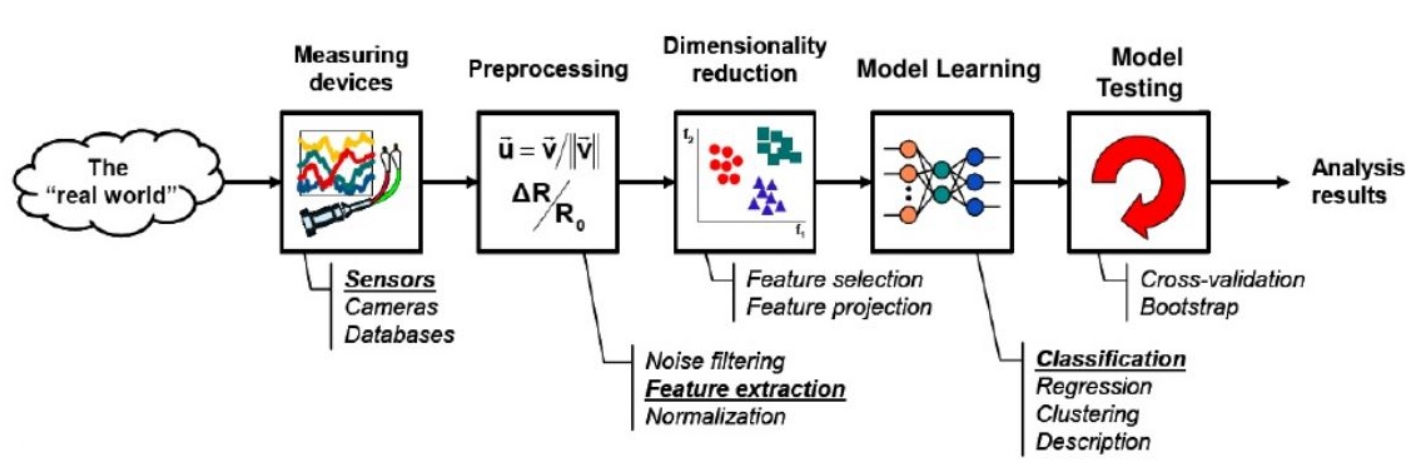
\includegraphics[width=\textwidth]{../img/Learning_process}
      \caption{Learning process in detail}
\end{figure}

\newpage

So, as can be observed in the image above, the learning process
in real-world applications where some kind of machine learning is
used is actually quite complex and it is also necessary to understand
how to perform each step of the pipeline shown below in order to build
an actually working machine learning model:

\begin{enumerate}
      \item \emph{\textbf{Data Source}}: This is the actual place where
            all data are generated. Normally this place is represented
            by the real world itself.
      \item \emph{\textbf{Data Collecting}}: This is the process by which
            all data are collected from the data source mentioned in
            point 1 by using different devices, such as
            \underline{sensors}, cameras, and databases.
      \item \emph{\textbf{Data Preprocessing}}: This is a process that
            depends on the type of the problem which is being addressed.
            Normally this process consists in some noise filtering, if the
            data are images or sensor signals, in normalization,
            if the data are seen as vectors, or in the
            so-called \emph{feature extraction}, which is achieved by
            transforming the data into a set of vectors containing relevant
            information.
      \item \emph{\textbf{Dimensionality Reduction(Optional)}}: Sometimes
            the features from the previous step are not used directly to
            produce a model, but are carefully selected to extract
            the most relevant part through the process called \emph{feature selection}.
      \item \emph{\textbf{Model Learning}}: This is the core step of the
            machine learning process in which, by applying a particular
            \emph{learning algorithm}, the actual \emph{model}
            is generated. The actual type of algorithm that will be
            applied depends on the particular nature of the problem being
            solved, such as classification, regression, clustering,
            description, and many others.
      \item \emph{\textbf{Model Testing}}: Once the model has been
            generated through a particular learning algorithm, a
            particular model testing protocol is applied to validate
            the accuracy of the generated model.
\end{enumerate}

It is also important to mention that another element that adds complexity
to the design of machine learning models is the choice of a particular
algorithm to use. This is because of the fact that there is a huge number
of machine learning algorithms that could be used. Fortunately, there is
always a guide that helps in making the right decision, that is the
particular nature of the problem to be solved.

At this point, given the general machine learning pipeline described
above, it is time to dive into the first most important element of
the process which is \emph{data}. The first
problem to solve is the fact that the concept of data is quite abstract,
but the concrete data that are used in real-world applications can be
extremely different form each other. For this reason, it is necessary to
define a general procedure that will allow representing data
independently of their actual structure. The answer to this problem is
called \emph{feature extraction}: that is the process by which each
\emph{example} in the \emph{training set} is associated with a data
structure, which is normally a simple vector of numbers with cardinality
n, that \emph{represents} the relevant information about the example and
indicates the \emph{actual form} that is seen by the algorithms. Each
such vector takes the name of \emph{feature vector}.

\newpage

One way of extracting these features is to consider them as
\emph{questions that can be asked} about the example, like for instance
in the image below with the fruits:

\vspace{5mm}

\begin{figure}[h]
      \centering
      \begin{subfigure}{0.40\textwidth}
            \centering
            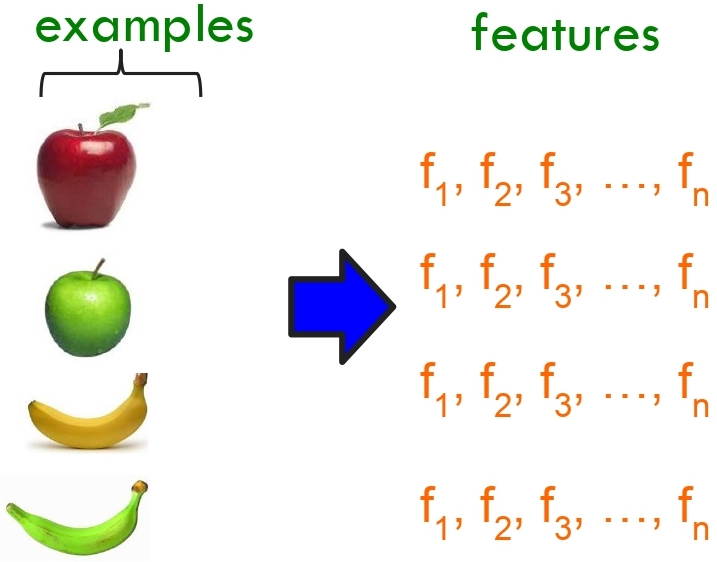
\includegraphics[width=\textwidth]{../img/Features_1}
      \end{subfigure}
      \hfill
      \begin{subfigure}{0.50\textwidth}
            \centering
            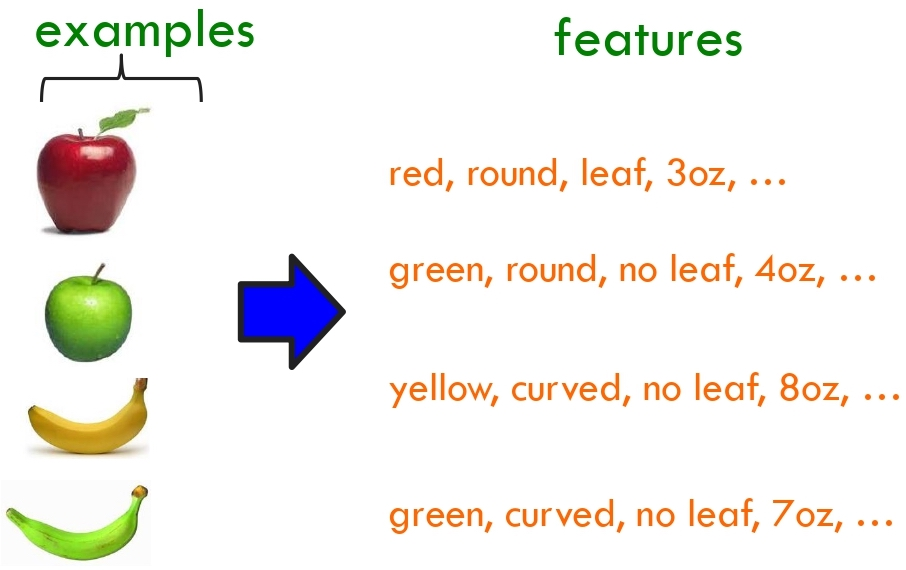
\includegraphics[width=\textwidth]{../img/Features_2}
      \end{subfigure}
      \caption{Example of features}
\end{figure}

\vspace{5mm}

Therefore, the final result of the feature extraction process is the
actual \emph{training set}, which is a set of numerical vectors, each of
which is the same dimension as the others. Unfortunately, there is a
problem with this approach, which is actually the most delicate part of
the design of the machine learning pipeline: \emph{how} are these
features chosen? There are actually many answers to this question and
the best answer should be the one that will ideally produce a set of
features that represent as well as possible the original data without
any loss of information. Therefore, there is always a risk that, after
processing the input data,
\underline{some information associated with the real data may be lost},
which in the case could cause the machine learning algorithm to work
improperly.

\subsection{Machine Learning Methods}

Now it is time to talk about different families of machine learning
methods to add a deeper understanding to what has been briefly
described in the overview subsection of these notes.

\subsubsection{Supervised Learning}

The first big family of machine learning methods is the so-called
\emph{Supervised Learning}. All methods associated with this family
have access to the data \emph{and} some annotations that are
associated with these data. These annotations are also called
\emph{labels}. Therefore, the training set, that is the input to the
learning algorithm, in these cases consists of a set of pairs, each of
which consists of an \emph{example}(in the form of a
\emph{feature vector}) and its relative \emph{label}. For this reason,
all the pairs in the training set are called \emph{labeled examples}.
Then this set of labeled examples is processed by the learning
algorithm to build a model, also called a predictor, that will be used
on new data, which have not been seen during the training phase, to
produce labels associated with these data. It is necessary to note that
all labels generated by the model will belong to the set of the
labels that have been learned from the training set. All this process
can be observed in the images below:

\newpage
% FIXME: resize the images below 

\begin{figure}[h]
      \centering
      \begin{subfigure}{0.45\textwidth}
            \centering
            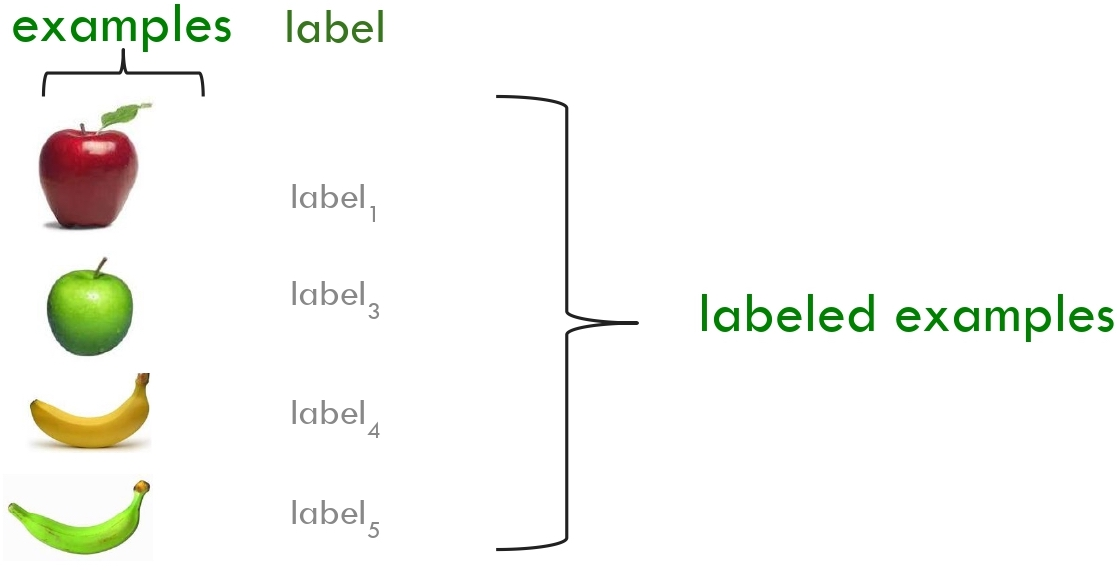
\includegraphics[width=\textwidth]{../img/Labeled_examples}
            \caption{Training Set}
      \end{subfigure}
      \hfill
      \begin{subfigure}{0.45\textwidth}
            \centering
            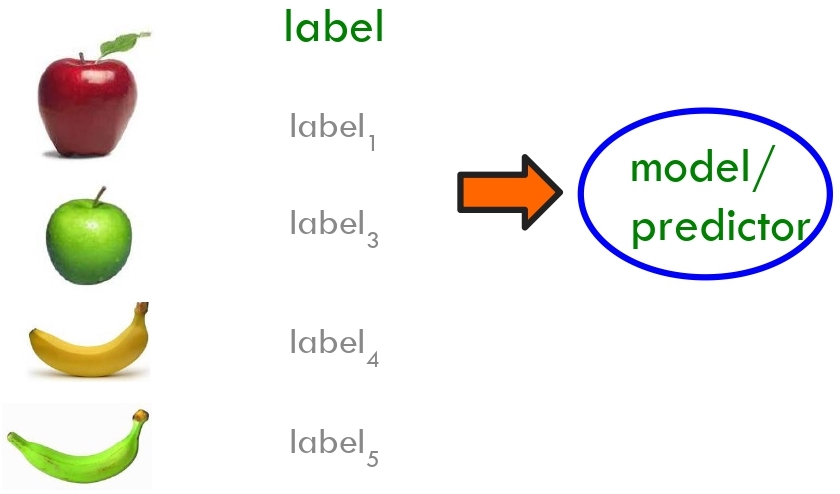
\includegraphics[width=\textwidth, height=0.55\textwidth]{../img/Supervised_training}
            \caption{Model Training}
      \end{subfigure}
      \hfill
      \begin{subfigure}{0.45\textwidth}
            \centering
            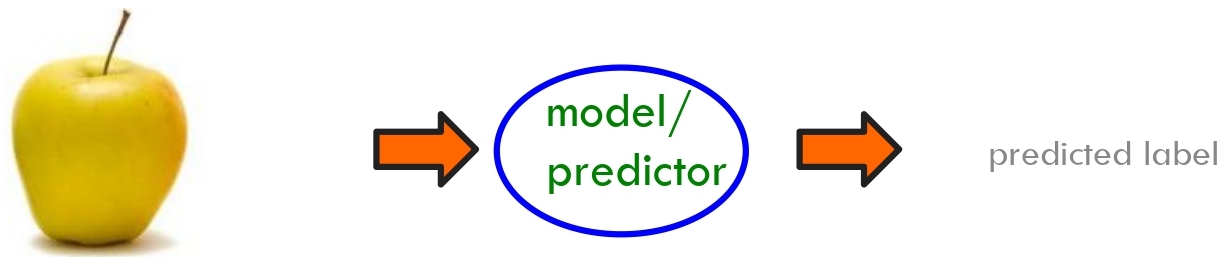
\includegraphics[width=\textwidth]{../img/Supervised_testing}
            \caption{Model Testing}
      \end{subfigure}
\end{figure}

\vspace{5mm}

At this point, it is possible to introduce some major machine learning
tasks that use the supervised learning structure defined above:

\begin{itemize}
      \item \emph{\textbf{Classification}}: Given a training set
            $\mathcal{T}=\{(x_1,y_1),...,(x_m,y_m)\}$ where
            $m$ is the total number of pairs of labeled examples,
            the task is to learn a function $f$, defined as
            $f : \mathbb{R}^d \rightarrow \{1,2,...,k\}$ where $d$
            is the dimension of the input space and $k$ is the
            \underline{finite} number of labels, to predict the label
            $y$ given the input $x$. So the dimension of the $x$
            component(feature vector) in the pairs of labeled examples
            and as input to the function $f$ is determined by the value
            of $d$, as can be observed in the examples below:

            \vspace{5mm}

            \begin{figure}[h]
                  \centering
                  \begin{subfigure}{0.52\textwidth}
                        \centering
                        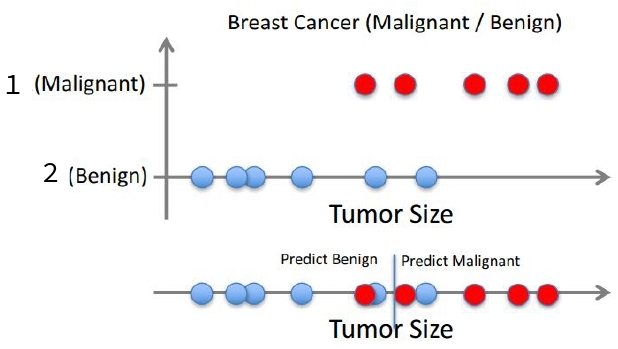
\includegraphics[width=\textwidth]{../img/Classification_1}
                        \caption{$x$ is one-dimensional($d=1$)}
                  \end{subfigure}
                  \hfill
                  \begin{subfigure}{0.38\textwidth}
                        \centering
                        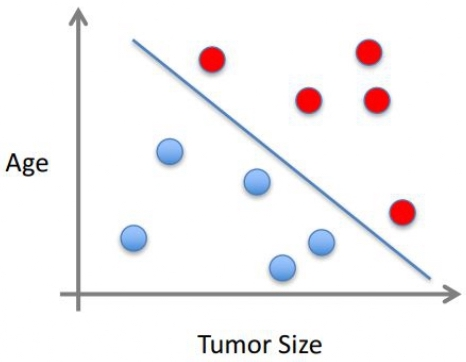
\includegraphics[width=\textwidth]{../img/Classification_2}
                        \caption{$x$ is multidimensional($d=2$)}
                  \end{subfigure}
            \end{figure}

            \vspace{5mm}

            This classification framework of supervised learning is of
            course extremely general and can be instantiated for
            several problems, such as Face Recognition, Character
            Recognition, Spam Detection, Medical Diagnosis, Biometrics
            and many others.

            \newpage

      \item \emph{\textbf{Regression}}: Given a
            training set $\mathcal{T}=\{(x_1,y_1),...,(x_m,y_m)\}$ where
            $m$ is the total number of pairs of labeled examples,
            the task is to learn a function $f$, defined as
            $f : \mathbb{R}^d \rightarrow \mathbb{R}$ where $d$
            is the dimension of the input space, to predict the label
            $y$ given the input $x$. As with Classification, the
            dimension of the $x$ component(feature vector) in the pairs
            of labeled examples and as input to the function $f$ is
            determined by the value of $d$. However, the big difference
            between Classification and Regression consists in the fact
            that all labels produced by the computed regression function
            are real-valued, so the set of all possible labels is
            \underline{not finite} by definition(i.e.\ it is
            \underline{continuous}). An example of regression is the
            following:

            \vspace{5mm}

            \begin{figure}[h]
                  \centering
                  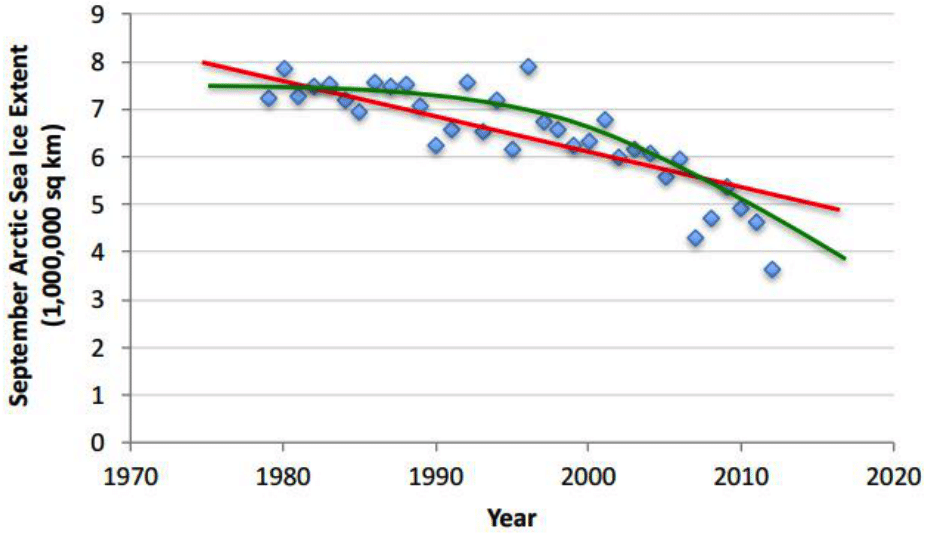
\includegraphics[width=0.7\textwidth]{../img/Regression_example}
                  \caption{Example of Regression}
            \end{figure}

            \vspace{5mm}

            As with Classification, this regression framework of
            supervised learning is of course extremely general
            and can be instantiated for several problems, such as
            Stock Value Prediction in Finance, Epidemiology, Car/Plane
            Navigation, Weather Forecasting in the area of Temporal
            Trends and many others.

      \item \emph{\textbf{Ranking}}: This is another supervised learning
            task in which all the labels in the training set and the ones
            generated by the computed ranking model are \emph{ranks},
            which are values indicating the sorting position/relevance
            of the elements. An example of ranking is search query
            evaluation in web browsers where, given a query and a set of
            web pages, a ranking is computed according to the ranks of
            the web pages, with the most relevant web sites appearing at
            the top. As with the previous two tasks, this ranking
            framework is extremely general and can be instantiated for
            several problems, such as User Preference(e.g.\ Netflix
            "My List" for movie queue ranking), Image Retrieval, Flight
            Search, Search in general and many others.
\end{itemize}

\newpage

\subsubsection{Unsupervised Learning}

The second big family of machine learning methods is the so-called
\emph{Unsupervised Learning}. As with supervised learning,
all methods associated with this family have access to the data
\emph{but} there are \emph{no} annotations associated with these data.
Therefore, the training set in this case consists only of a set
of \emph{examples}(always in the form of \emph{feature vectors})
without any associated labels. Then this set of examples is processed
by the learning algorithm to build a model consisting of a
\emph{hidden structure} behind the input data.

At this point, it is possible to introduce some major machine learning
tasks that use the unsupervised learning structure:

\begin{itemize}
      \item \emph{\textbf{Clustering}}: Given a training set
            $\mathcal{T}=\{x_1,...,x_m\}$ where m is the total number
            of examples, the task is to output a hidden structure
            behind the input data. In this particular case the
            discovered structure is represented by the so-called
            \emph{clusters}, which are perfectly illustrated in the
            following image:

            \vspace{5mm}

            \begin{figure}[h]
                  \centering
                  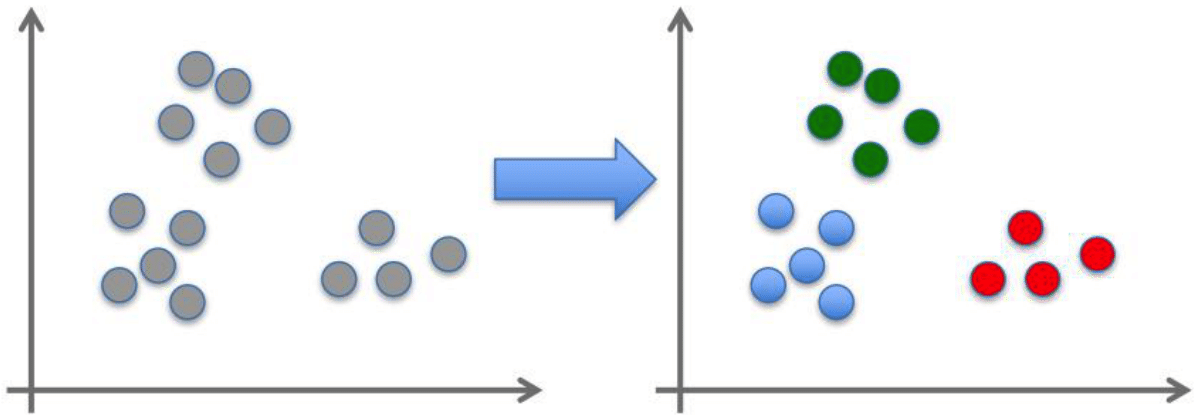
\includegraphics[width=0.8\textwidth]{../img/Clustering_example}
                  \caption{Example of Clustering}
            \end{figure}

            \vspace{5mm}

            This clustering framework of unsupervised learning is of
            course extremely general and can be instantiated for
            several problems, such as Social Network Analysis, Genomics,
            Image Segmentation and many others.

      \item \emph{\textbf{Anomaly Detection}}: This is another
            unsupervised learning task in which the training set consists
            of events or objects and the task consists in detecting those
            events or objects that are unusual or atypical.

            This anomaly detection framework of unsupervised learning
            is of course extremely general and can be instantiated for
            several problems, such as Credit Card Fraud Detection,
            Video Surveillance and many others.

            \newpage

      \item \emph{\textbf{Dimensionality Reduction}}: This is another
            unsupervised learning task in which the training set consists
            of data characterized by a certain number of dimensions
            (i.e.\ variables) and the task is to reduce these dimensions
            in order to get a set of data characterized by a reduced
            number of variables while preserving the most important
            relationships between the data as they were in the initial
            set. This particular task can be observed in the following
            image:

            \vspace{5mm}

            \begin{figure}[h]
                  \centering
                  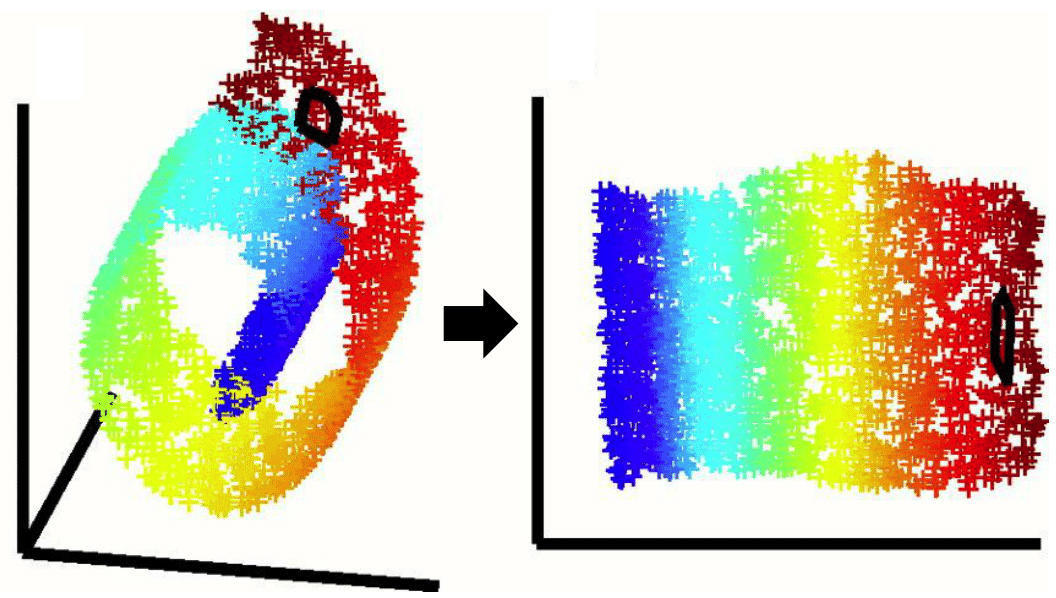
\includegraphics[width=0.45\textwidth]{../img/Dim_reduction_example}
                  \caption{Example of Dimensionality Reduction}
            \end{figure}

            \vspace{5mm}

            This dimensionality reduction framework of unsupervised
            learning is of course extremely general and can be
            instantiated for several problems, such as Output Inspection
            in the case of a classification algorithm and many others.
\end{itemize}

\subsubsection{Reinforcement Learning}

The third big family of machine learning methods is the so-called
\emph{Reinforcement Learning}. The big difference between this
family and the previous two consists in the fact that there is no
training set in reinforcement learning but there is only a numerical
performance score as its guidance. Therefore, in this case there is a
totally different learning scheme, which is based on the following idea:
an \emph{agent} learns from an \emph{environment} by interacting with
it through some \emph{actions} that make it receive \emph{rewards}
and make it modify its current \emph{state}. This idea is clearly
illustrated in the following image:

\vspace{2mm}

\begin{figure}[h]
      \centering
      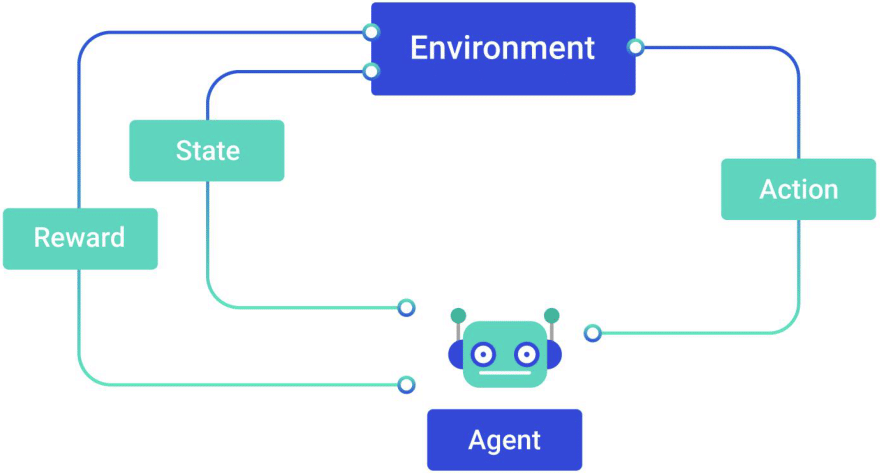
\includegraphics[width=0.5\textwidth]{../img/Reinforcement_learning}
      \caption{Reinforcement Learning Scheme}
\end{figure}

\vspace{5mm}

\newpage

It immediately becomes clear that this learning scheme is highly
\emph{interactive} because the agent, in order to learn some useful
information, continuously completes \emph{sequences of states/examples}
and gets \emph{rewards} after completing those sequences. In this way,
based on the values of the rewards, the agent learns to predict the
\emph{action} to take for each individual state/example in order to
achieve its final goal, which is an optimal, or nearly-optimal, way to
maximize the amount of gained rewards. An example of a sequence evaluation
is illustrated in the following image:

\vspace{5mm}

\begin{figure}[h]
      \centering
      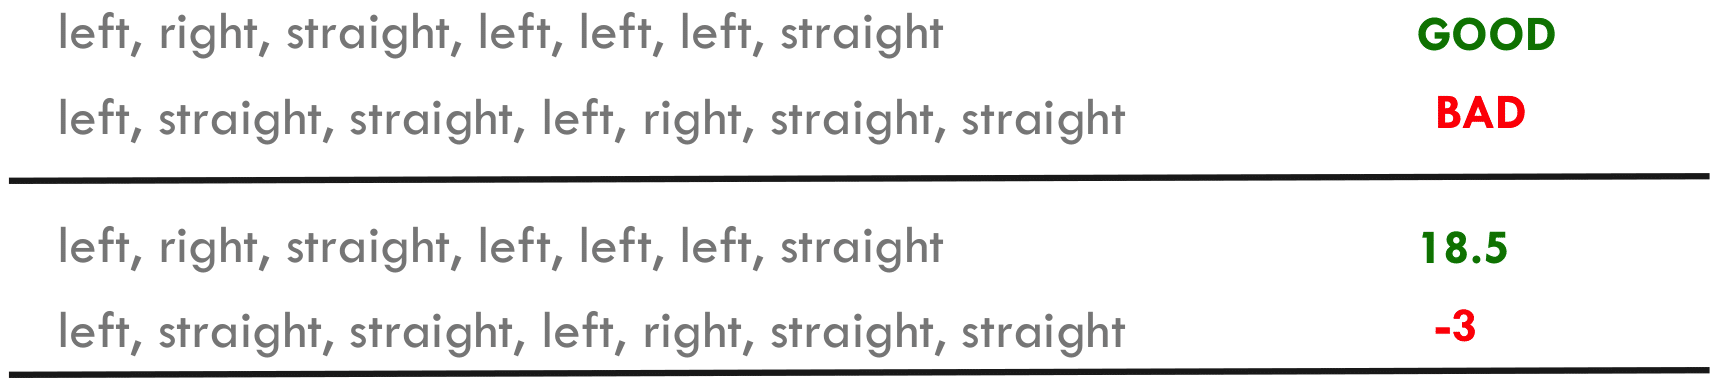
\includegraphics[width=0.8\textwidth]{../img/Sequence_example}
      \caption{Example of a sequence evaluation}
\end{figure}

\vspace{5mm}

Some famous examples of the application of reinforcement learning are
for instance the Backgammon and Go board games and the computer game
Atari Breakout, in which you try to learn winning sequences.

\subsubsection{Other Learning Variations}

Besides the three largest families of machine learning methods,
there are other families that will not be covered in these notes.
However, it is always useful to mention \emph{some} of them because
of their usage in different areas:

\begin{itemize}
      \item \emph{\textbf{Semi-supervised Learning}}: This is a family
            of hybrid machine learning methods that involve small
            datasets of labeled examples(supervised learning) and large
            datasets of examples that don't contain any
            labels(unsupervised learning).

            \vspace{5mm}

            \begin{figure}[h]
                  \centering
                  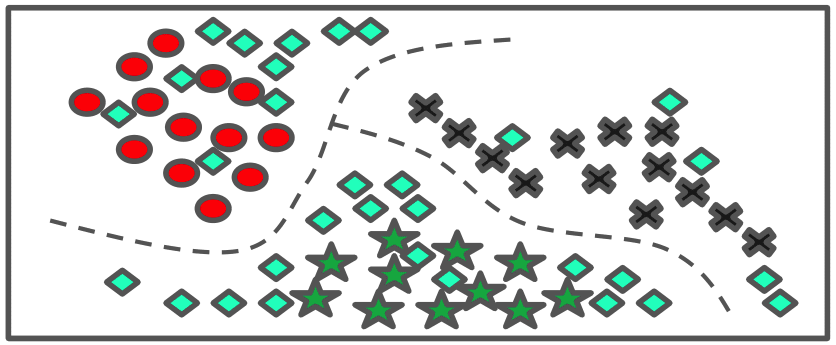
\includegraphics[width=0.6\textwidth]{../img/Semi_supervised_learning}
                  \caption{Example of Semi-supervised Learning}
            \end{figure}

            \vspace{5mm}

            \newpage

      \item \emph{\textbf{Active Learning}}: This is a family of machine
            learning methods that are characterized by an incremental
            learning scheme and by some human supervision(some useful
            feedback) which is involved only in the case of the most
            difficult examples.

            \vspace{5mm}

            \begin{figure}[h]
                  \centering
                  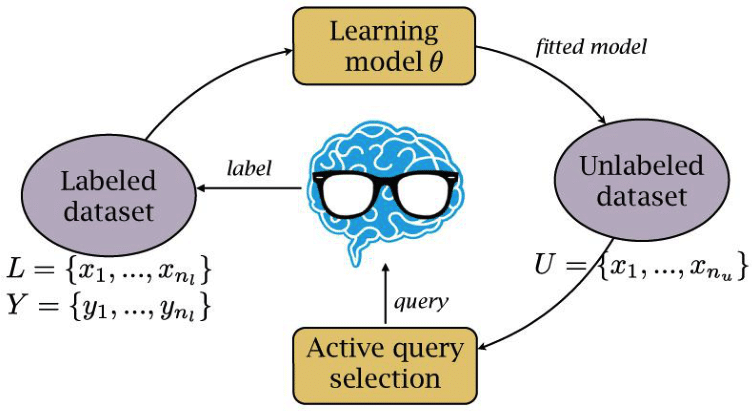
\includegraphics[width=0.55\textwidth]{../img/Active_learning}
                  \caption{Example of Active Learning}
            \end{figure}

            \vspace{5mm}
\end{itemize}

\noindent Some learning variations also derive from \emph{how} the data
are retrieved:

\begin{itemize}
      \item \emph{\textbf{Online Learning}}: There is a continuous
            process during which the incoming data are immediately
            used to update the model.

      \item \emph{\textbf{Offline Learning}}: The data, such as training
            sets, are available offline and are used to train a model
            that will then be used on new unknown data.
\end{itemize}

\noindent Other learning variations also derive from the \emph{type} of
a model:

\begin{itemize}
      \item \emph{\textbf{Generative vs Discriminative Learning}}:
            These two different types will be covered in the
            particular case of supervised learning later in these notes.
      \item \emph{\textbf{Parametric vs Non-parametric Learning}}:
            Some models may or may not contain some parameters that
            are learned during the training phase.
\end{itemize}

\subsection{Intro to Data Generating Distributions}

Now it is time to talk more deeply about one of the most relevant
and critical elements of machine learning, that is \emph{features}
and their \emph{generation}. As mentioned previously, the training
set is made of examples(labeled in the case of supervised learning)
that are represented in the form of features and then the model,
that is generated during the training phase, makes predictions
\textbf{based on these features}. The testing set is also made of
examples that are represented in the form of features, but in this
case, no answers are provided, since the answers will be generated by
the model, which will process the features of each example to produce
the predictions(labels in the case of supervised learning).

\newpage

The natural question that arises from this summary is how the training
and testing sets should be generated. The natural answer to this
question is that \textbf{the same feature extraction algorithm}
should be applied to generate both the training and testing sets, but
this is not enough. The fact is that the result of a prediction will
strongly depend on the features that have been seen, so the examples in
the testing set should contain features that are \emph{similar} to some
features in some examples in the training set. This is an intuition that
has to be formalized and satisfied in order to be able to
\textbf{generalize from the training set}. So the implicit
assumption here is that the examples in the testing set are
\emph{in some way similar} to the examples in the training set.
This is not always the case, but sometimes it will be necessary
to assume that it is.

At this point, it is necessary to formalize the intuition described
above and this can be achieved by modeling the similarity between
the training and testing sets through a \emph{probabilistic model}
of learning. This probabilistic modeling implies
\textbf{the most important assumption of machine learning},
that is the fact that \textbf{it is possible to learn} because it is
\textbf{assumed} that \textbf{both} the training
\textbf{and} testing sets are generated based on the \textbf{same}
underlying probability distribution, which is \textbf{unknown} and
called in this context \textbf{Data Generating Distribution(DGD)}.
So, thanks to this assumption, it is possible to build systems that
can generalize between the training and testing sets by starting to
consider the different features of the examples in the training
and testing sets in terms of probability, as can be observed in the
following image:

\vspace{5mm}

\begin{figure}[h]
      \centering
      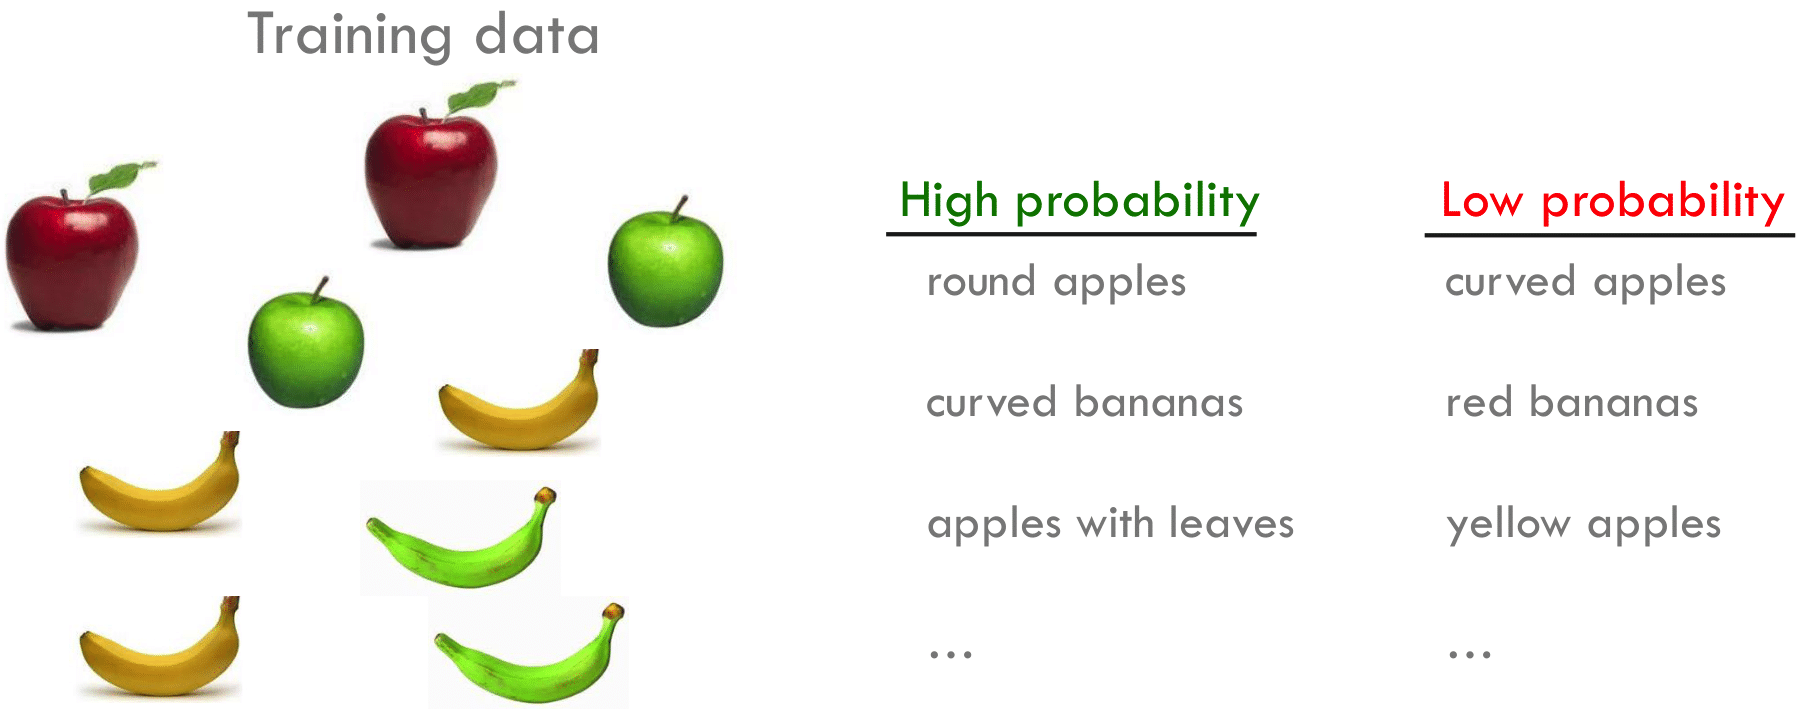
\includegraphics[width=0.6\textwidth]{../img/Testing_set_prob}
      \caption{Example of probability values}
\end{figure}

\vspace{5mm}

In order to start getting familiar with the concept of data generating
distribution it could be useful to observe the following image, which
represents a data generating distribution with different
\emph{likelihood values of sampling}, for every fruit category,
in terms of different amounts of fruits:

\newpage

\begin{figure}[h]
      \centering
      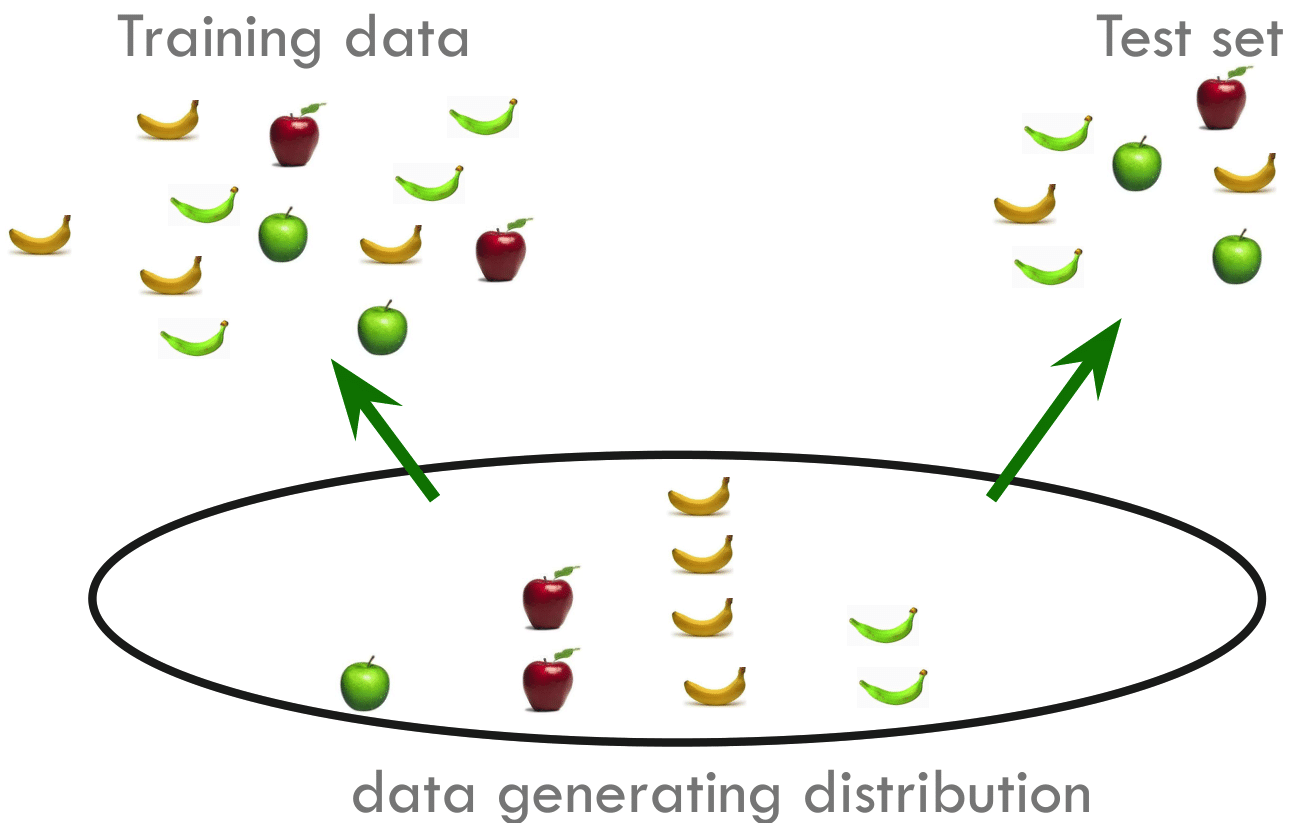
\includegraphics[width=0.6\textwidth]{../img/DGD_example}
      \caption{Example of a DGD}
\end{figure}

\vspace{5mm}

It is also extremely useful to observe some counterexamples that
clarify even more the importance of the fact that both the training
and testing sets must be generated based on the same probability
distribution:

\vspace{5mm}

\begin{figure}[h]
      \begin{subfigure}{0.45\textwidth}
            \centering
            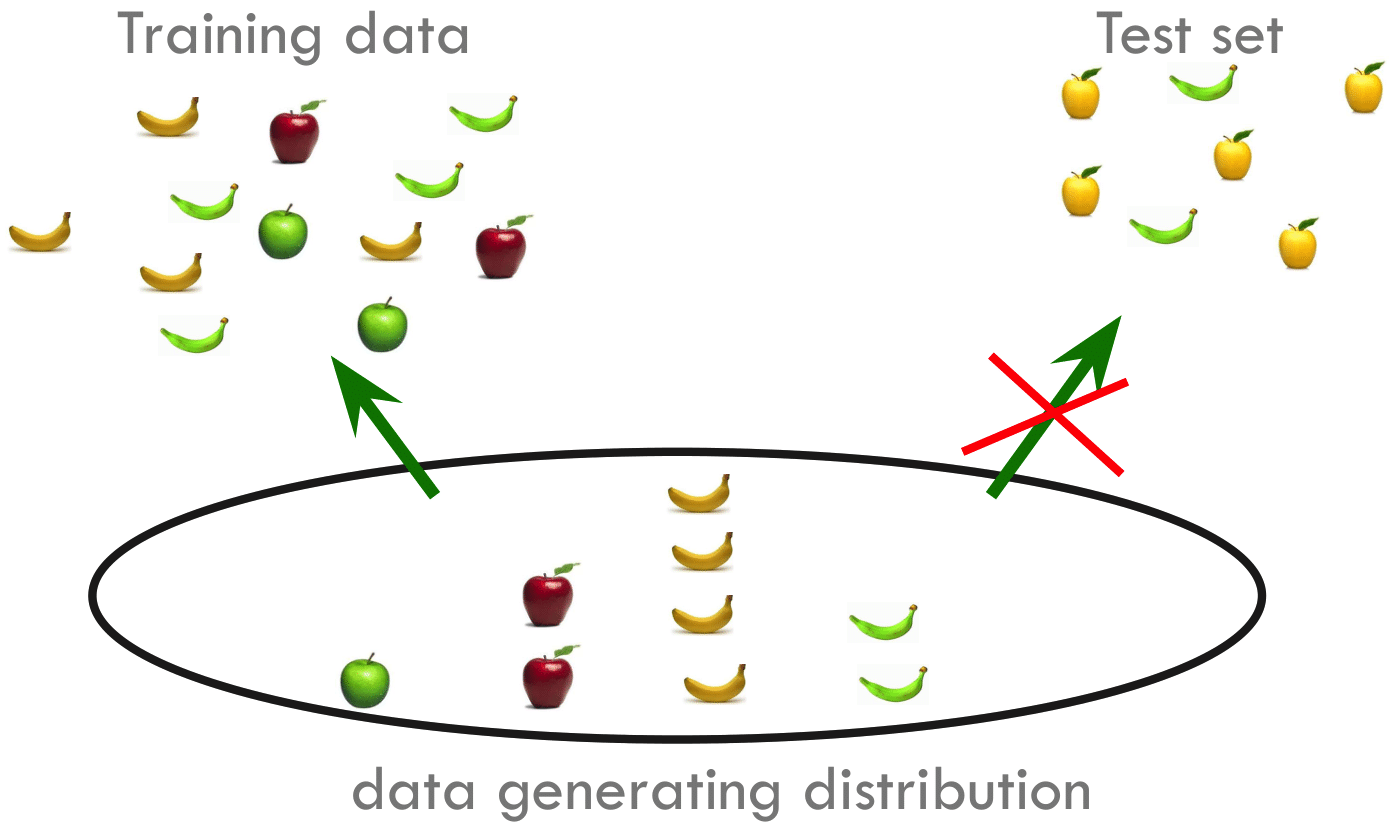
\includegraphics[width=\textwidth]{../img/DGD_counterexample_1}
            \caption{Testing Set with new fruits}
      \end{subfigure}
      \hfill
      \begin{subfigure}{0.45\textwidth}
            \centering
            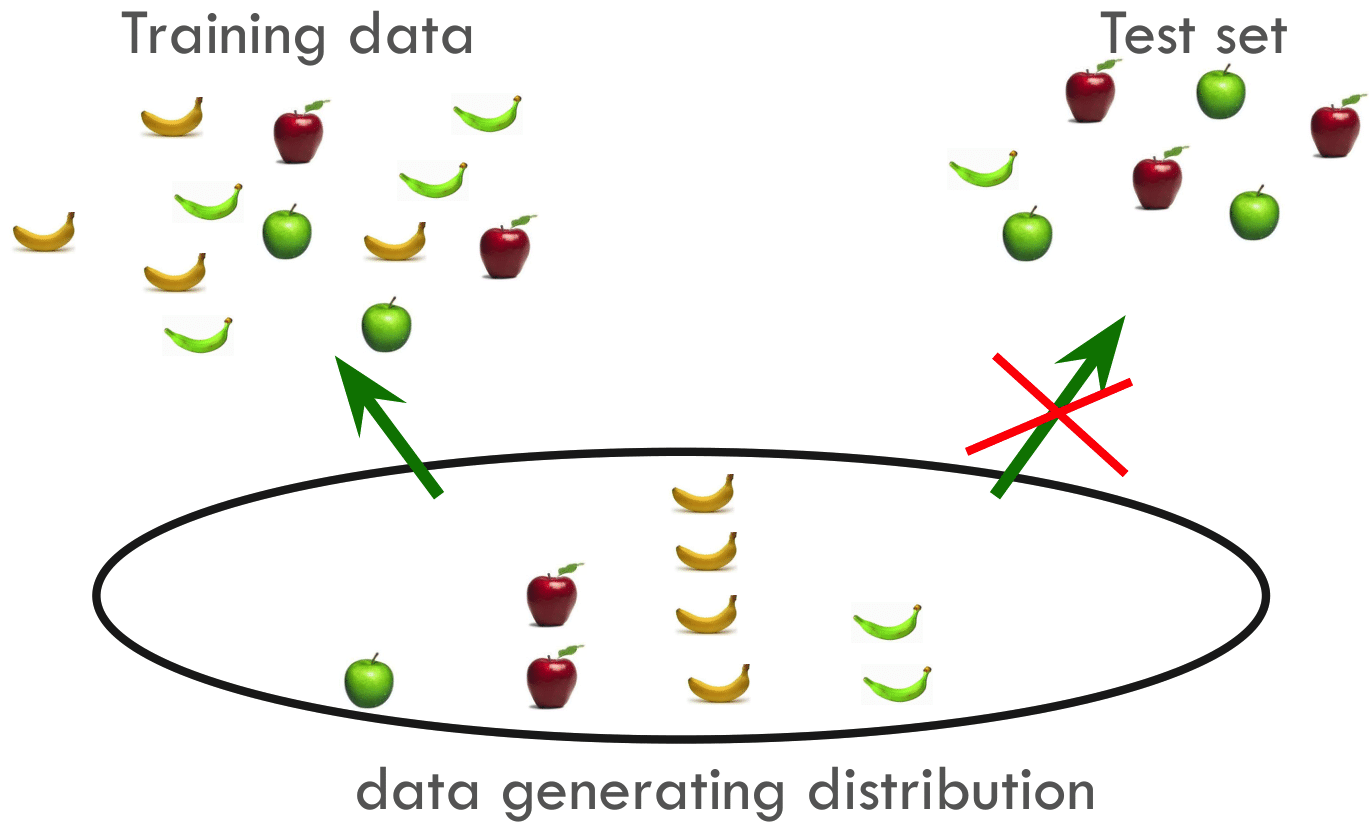
\includegraphics[width=\textwidth]{../img/DGD_counterexample_2}
            \caption{Testing Set without bananas}
      \end{subfigure}
      \caption{Training and Testing Sets generated by different DGDs}
\end{figure}

\subsection{Applied Machine Learning}

In this subsection, the refined version of the machine learning process
will be presented, with a particular attention on its usage in real-world
applications. So, the following are the five main ingredients to build a
working machine learning system:

\begin{itemize}
      \item \emph{\textbf{Task}}: First of all, it is necessary to formalize
            the task that is being solved into one of the common tasks of
            machine learning, for example when the task of recognizing
            a bird in a photo becomes a classification task, which is well-known
            in machine learning.
      \item \emph{\textbf{Data}}: It is always crucial to have a proper set of
            data in order to correctly solve a given task. The importance of
            data in machine learning will always be a fundamental aspect of the
            whole process.
      \item \emph{\textbf{Model and Hypothesis Space}}: In general, it is always
            possible to choose, from a large family of machine learning models,
            a particular model structure that will be suitable for the task.
      \item \emph{\textbf{Objective Function}}: It is always necessary to define an objective
            function that is directly related to the performance measurement of the
            chosen model.
      \item \emph{\textbf{Learning Algorithm}}: Based on the choice of a particular
            model and performance measurements given by the objective function, it
            is possible to apply some machine learning algorithm in order to produce
            the desired model.
\end{itemize}

At this point, it is useful to dive into each of the five elements mentioned above
in order to understand more clearly the importance of their roles.

\subsubsection{Task}

In general a task can be identified with a \emph{set of functions}
$\mathcal{F}_{task} \subset \mathcal{Y}^{\mathcal{X}}$, where ${\mathcal{X}}$
is the input space and ${\mathcal{Y}}$ is the output space,
that can potentially solve a problem. So it consists of functions, in the form of
$f : {\mathcal{X}} \rightarrow {\mathcal{Y}}$, which assign an input
$x \in \mathcal{X}$ an output $y \in \mathcal{Y}$. Obviously, the nature of
$\mathcal{X}, \mathcal{Y}$ and $\mathcal{F}_{task}$ will depend on the type of task
to be solved, as can be observed from the tasks formalized below:

\begin{itemize}
      \item \emph{\textbf{Classification}}: The output space $\mathcal{Y}$ is
            discrete, so each input $x \in \mathcal{X}$ is mapped through the function
            $f$ onto $f(x) \in \mathcal{Y}=\{c_1,...,c_k\}$.
      \item \emph{\textbf{Regression}}: The output space $\mathcal{Y}$ is continuous,
            so each input $x \in \mathcal{X}$ is mapped through the function $f$
            onto $f(x) \in \mathcal{Y} \subseteq \mathbb{R}$.
      \item \emph{\textbf{Density Estimation}}: An unsupervised learning task that
            consists in calculating the underlying probability distribution
            $f \in \Delta(\mathcal{X})$ over the data in $\mathcal{X}$.
      \item \emph{\textbf{Clustering}}: An unsupervised learning task that consists
            in calculating a function $f \in \mathbb{N}^{\mathcal{X}}$ that assigns
            each input $x \in \mathcal{X}$ a cluster index $f(x) \in \mathbb{N}$, so
            all points that are mapped to the same index form a cluster.
      \item \emph{\textbf{Dimensionality Reduction}}: An unsupervised learning task
            that consists in calculating a function $f \in \mathcal{Y}^{\mathcal{X}}$
            that maps each higher dimensional input $x \in \mathcal{X}$ to a lower
            dimensional embedding $f(x) \in \mathcal{Y}$, where
            $dim(\mathcal{Y}) \ll dim(\mathcal{X})$.
\end{itemize}

\subsubsection{Data}

Different types of tasks can be performed on different types of data, which can vary
from movie records taken from IMDb or environmental changes registered and collected by
electronic devices to a simple collection of fruits. The important aspect here is the fact
that all these significantly different types of data are represented in the same way,
that is, in terms of their most important characteristics, which are called
\emph{features}. Therefore, these features, which are normally grouped into vectors,
represent how the input data are actually visualized by machine learning algorithms.
Unfortunately, as explained earlier, this feature extraction process almost always
results in a loss of information about the original form of the data.

Besides the formal way of representing data in terms of vectors of features, the other
extremely important concept about data is the so-called \emph{data generating distribution}.
This data generating distribution is generally \emph{unknown} and represents a distribution
of probabilities by which the data are generated. From this point of reading onwards,
the data generating distribution will be called $p_{data}$ and will be formally defined
as follows:

\begin{itemize}
      \item \emph{\textbf{Classification and Regression}}:
            \begin{equation*}
                  p_{data} \in \Delta(\mathcal{X} \times \mathcal{Y})
            \end{equation*}
      \item \emph{\textbf{Density Estimation, Clustering and Dimensionality Reduction}}:
            \begin{equation*}
                  p_{data} \in \Delta(\mathcal{X})
            \end{equation*}
\end{itemize}

Since this data generating distribution is unknown, the only way to access it is through
\emph{sampling}. So, in practice it is assumed that training data, validation data and test
data are generated through sampling from the same underlying probability distribution and
only in a similar case the final model will probably work well. A typical machine learning
pipeline in which the assumption about the data generating distribution is satisfied can be
observed in the image below:

\vspace{5mm}

\begin{figure}[h]
      \centering
      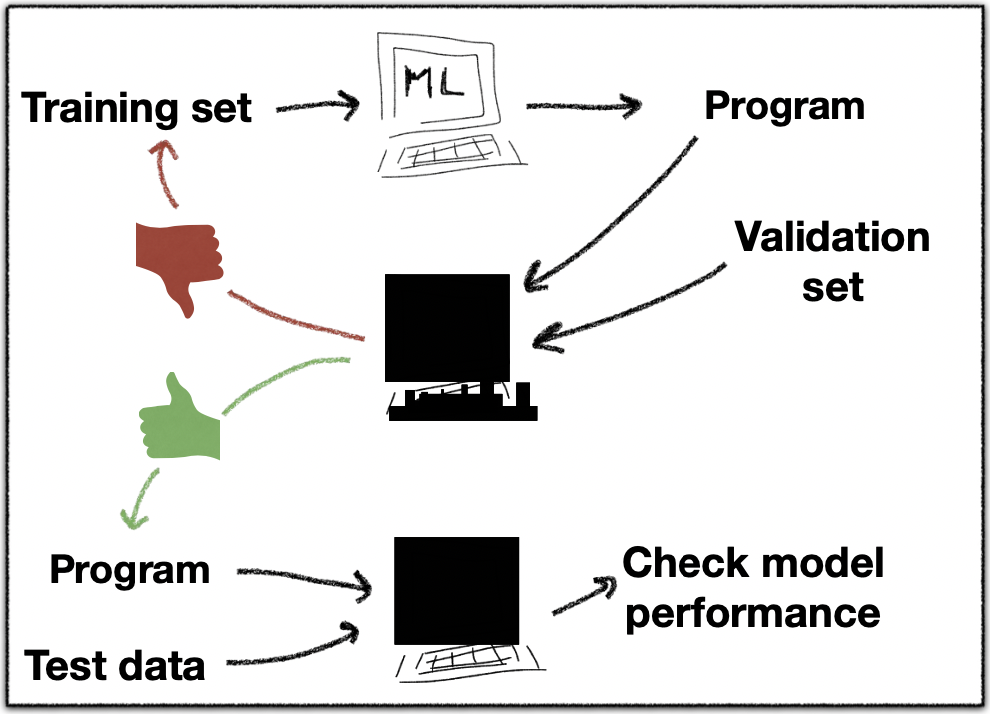
\includegraphics[width=0.6\textwidth]{../img/Train_Validate_Test}
      \caption{Practical Machine Learning Pipeline}
\end{figure}

\newpage

In machine learning, besides the importance of the feature extraction process and the assumption about
the data generating distribution of the datasets, a particular role is also played by the so-called
\textbf{Training Set Design}. This aspect is particularly important because the failure of a
machine learning algorithm is often caused by a bad selection of training samples. The issue is that
sometimes some unwanted correlations are introduced into the dataset, from which the algorithm could
derive wrong conclusions. This problem is perfectly described by the following probably invented
story:

\vspace{5mm}

\begin{figure}[h]
      \centering
      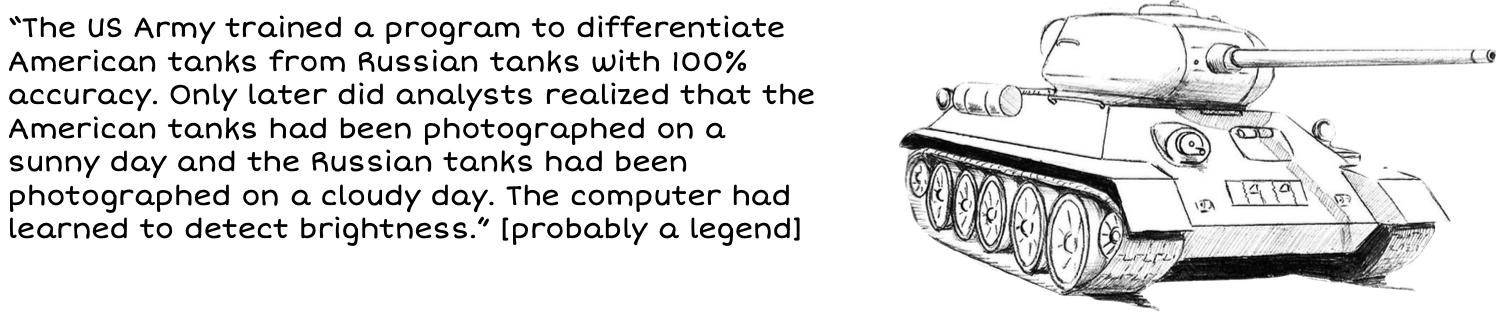
\includegraphics[width=0.8\textwidth]{../img/Train_Failure}
      \caption{Why the training set design is so important}
\end{figure}

\subsubsection{Model and Hypothesis Space}

At this point, once the task has been identified and the datasets have been properly built,
it is necessary to talk about the next two key concepts that are called \textbf{Model} and
\textbf{Hypothesis Space}. The model is basically a \emph{program} that solves the task, so
it is the \emph{implementation} of the above-mentioned function $f \in \mathcal{F}_{task}$
that can be tractably computed. The hypothesis space is a \emph{set of models}
$\mathcal{H} \subset \mathcal{F}_{task}$ where a particular learning algorithm seeks a
solution, that is, a model. So, in general, the set of models from which to choose is a
subset of all possible models that could solve a given task, since the number of all possible
algorithms and consequently of all possible models produced by these algorithms is
particularly big and it should be clear that some algorithms are yet to be discovered.
The following image perfectly describes what has just been explained:

\begin{figure}[h]
      \centering
      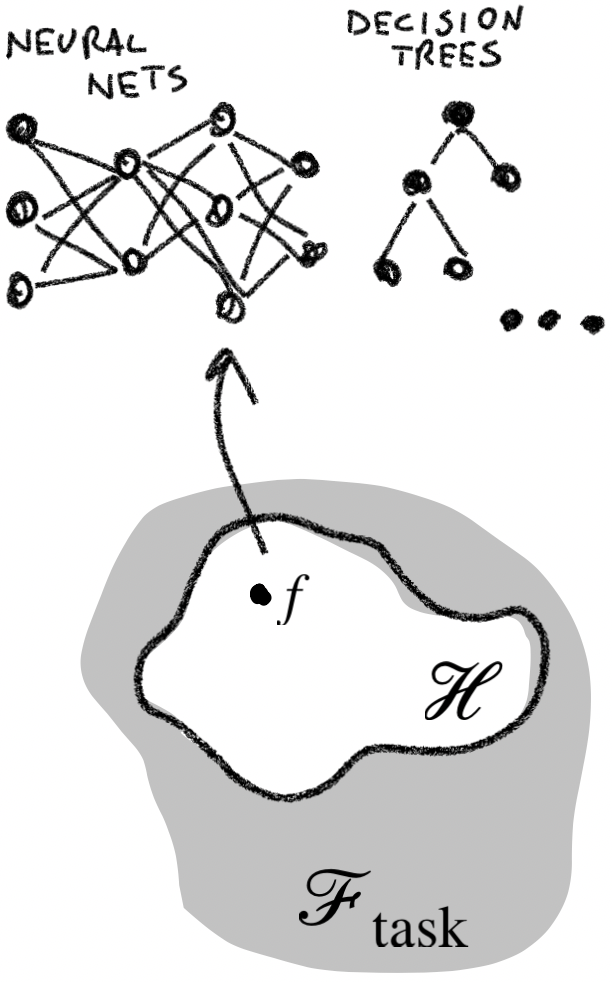
\includegraphics[width=0.23\textwidth]{../img/Model_and_hypothesis_space}
      \caption{Model and Hypothesis Space}
\end{figure}

\newpage

From the formal and practical point of view, for example in the case of
\emph{Polynomial Curve Fitting}, the general form of a model that solves a given
task is the following:

\begin{equation*}
      f_w(x) = \sum_{j = 0}^{M} w_jx^j
\end{equation*}

So, the learning process, in this case, consists in discovering the
\emph{best function} $f$(at this point of reading it is not clear what this means),
which actually means that the learning process consists in discovering the
\emph{best parameters} $\{w_0,...,w_M\}$ of that function.

The hypothesis space, on the other hand, is formally defined as follows:

\begin{equation*}
      \mathcal{H}_M = \{f_w : w \in \mathbb{R}^M\}
\end{equation*}

This means that the hypothesis space is the set of all those functions, parameterized on
values $w_0,...,w_M$, which, for some \emph{fixed} polynomial degree $M \in \mathbb{N}$,
solve the given task. An example of different polynomial models with different degrees
can be observed in the image below:

\begin{figure}[h]
      \centering
      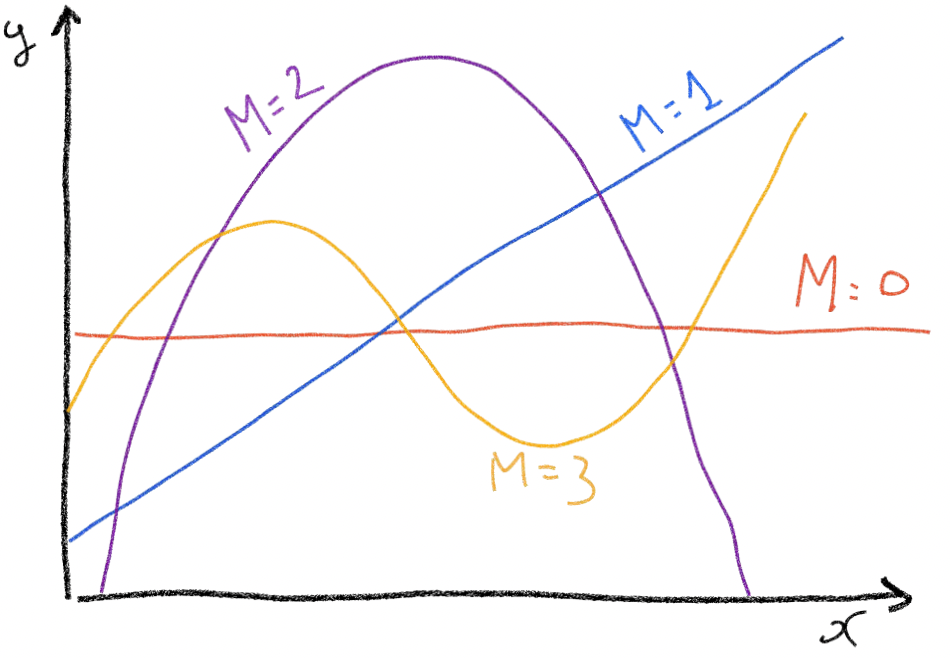
\includegraphics[width=0.4\textwidth]{../img/Polynomial_models}
      \caption{Polynomial Models}
\end{figure}

\subsubsection{Objective Function}

At this point, it is necessary to mathematically formalize the abstract property of
a model of being the best choice to make among all possible models and this is
done by introducing the concept of \textbf{Generalization Error Function} $E(f; p_{data})$
that determines how well a solution $f \in \mathcal{F}_{task}$ fits some given data.
So, this particular objective function basically guides the selection of
\emph{the best ideal solution} in $\mathcal{F}_{task}$. This best ideal solution is
formally defined as follows:

\begin{equation*}
      f^* \in \arg \min_{f \in \mathcal{F}_{task}} E(f; p_{data})
\end{equation*}

An example of the best ideal solution to a given task can be observed in the following image:

\newpage

\begin{figure}[h]
      \centering
      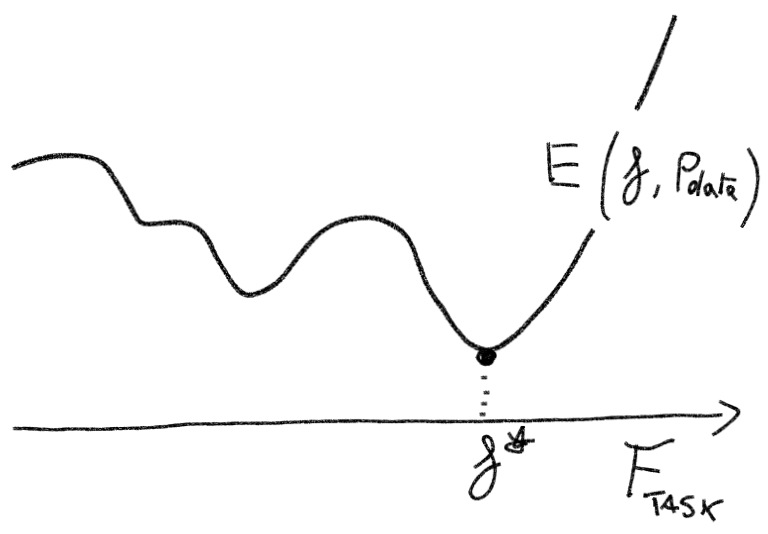
\includegraphics[width=0.4\textwidth]{../img/Best_ideal_model}
      \caption{Best Ideal Model in $\mathcal{F}_{task}$}
\end{figure}

Unfortunately, the biggest problem with this approach is the fact that \textbf{the search
      space $\mathcal{F}_{task}$ is too large and the data generating distribution
      $p_{data}$ is unknown}, so there is no available procedure that would allow calculating
the best ideal model. This is the reason why, at first, it is necessary to
restrict the search space $\mathcal{F}_{task}$ to the hypothesis space
$\mathcal{H} \subset \mathcal{F}_{task}$ and then to calculate the best solution
that can be implemented and evaluated in a tractable way within this restricted space,
always be considering the same objective function $E(f; p_{data})$.
In this way, \emph{the best feasible solution} would be formally defined as follows:

\begin{equation*}
      f_{\mathcal{H}}^* \in \arg \min_{f \in \mathcal{H}} E(f; p_{data})
\end{equation*}

An example of the best feasible solution found within the hypothesis space can be observed
in the following image:

\begin{figure}[h]
      \centering
      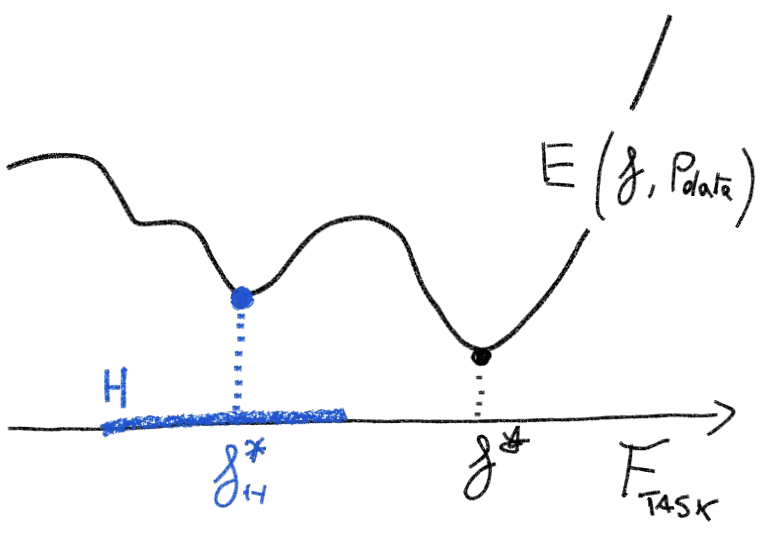
\includegraphics[width=0.4\textwidth]{../img/Best_feasible_model}
      \caption{Best Feasible Model in $\mathcal{H}$}
\end{figure}

Unfortunately, even in this case it is impossible to calculate the best solution,
since \textbf{the data generating distribution $p_{data}$ is still unknown}. This
is the reason why it is necessary to work only on a set of observations that are
\emph{sampled} from the data generating distribution, that is, a \textbf{Training Set}
$\mathcal{D}_n = \{z_1,...,z_n\}$ with $z_i \sim p_{data}$, where in the case of
polynomial curve fitting $z_i = (x_i,y_i) \in \mathcal{X} \times \mathcal{Y}$.
In this way, \emph{the best actual solution} would be formally defined as follows:

\newpage

\begin{equation*}
      f_{\mathcal{H}}^*(\mathcal{D}_n) \in \arg \min_{f \in \mathcal{H}} E(f; \mathcal{D}_n)
\end{equation*}

Moreover, in this case it is no longer possible to consider the same objective
function, but it is necessary to introduce a new objective function $E(f; \mathcal{D}_n)$,
which is called \textbf{Training Error Function}. The important aspect here is that
the two error functions should be as similar as possible.

An example of the best actual solution found within the hypothesis space can be observed
in the following image:

\begin{figure}[h]
      \centering
      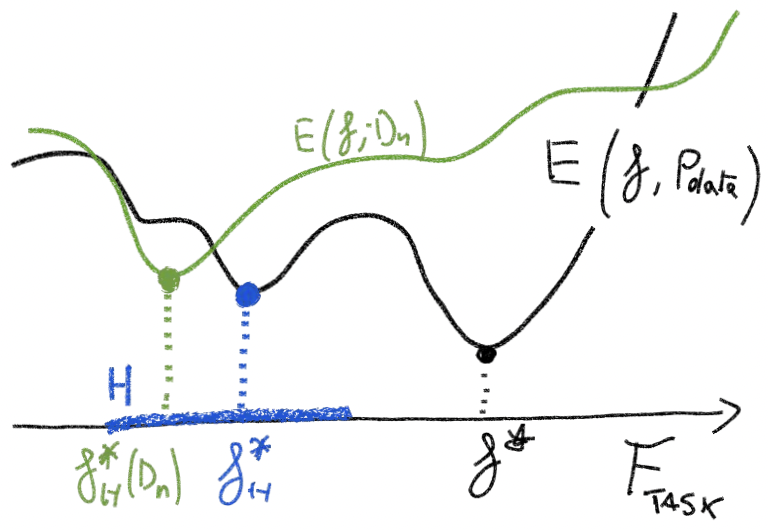
\includegraphics[width=0.4\textwidth]{../img/Best_actual_model}
      \caption{Best Actual Model in $\mathcal{H}$}
\end{figure}

At this point, it is possible to dive into the actual mathematical form that the
generalization and training error functions have. Typically the generalization and
training error functions can be written in terms of a \textbf{pointwise loss function}
$l(f;z)$ measuring the error incurred by $f$ on the training example $z$. So, the two
functions would have following forms:

\begin{equation*}
      E(f; p_{data}) = \mathbb{E}_{z \sim p_{data}}[l(f;z)]
\end{equation*}

and

\begin{equation*}
      E(f; \mathcal{D}_n) = \frac{1}{n} \sum_{i = 1}^{n} l(f;z_i)
\end{equation*}

This pointwise loss function is basically computed by comparing the prediction $f(x)$
of the model, associated with the input $x$, and the so-called \textbf{ground truth}
$z$, also associated with the input $x$. It is also important to notice that there are
several possible implementations of this pointwise loss function, which will be
analyzed later in these notes. For example, in the case of polynomial curve fitting,
the implementation of the pointwise loss function $l(f;z_i) = l(f;(x_i,y_i))$ is
$[f(x_i) - y_i]^2$, so the training error function becomes as follows:

\begin{equation*}
      E(f; \mathcal{D}_n) = \frac{1}{n} \sum_{i = 1}^{n} [f(x_i) - y_i]^2
\end{equation*}

and takes the name of \textbf{Mean Squared Error}. The meaning of this particular
implementation can be observed in the following image:

\newpage

\begin{figure}[h]
      \centering
      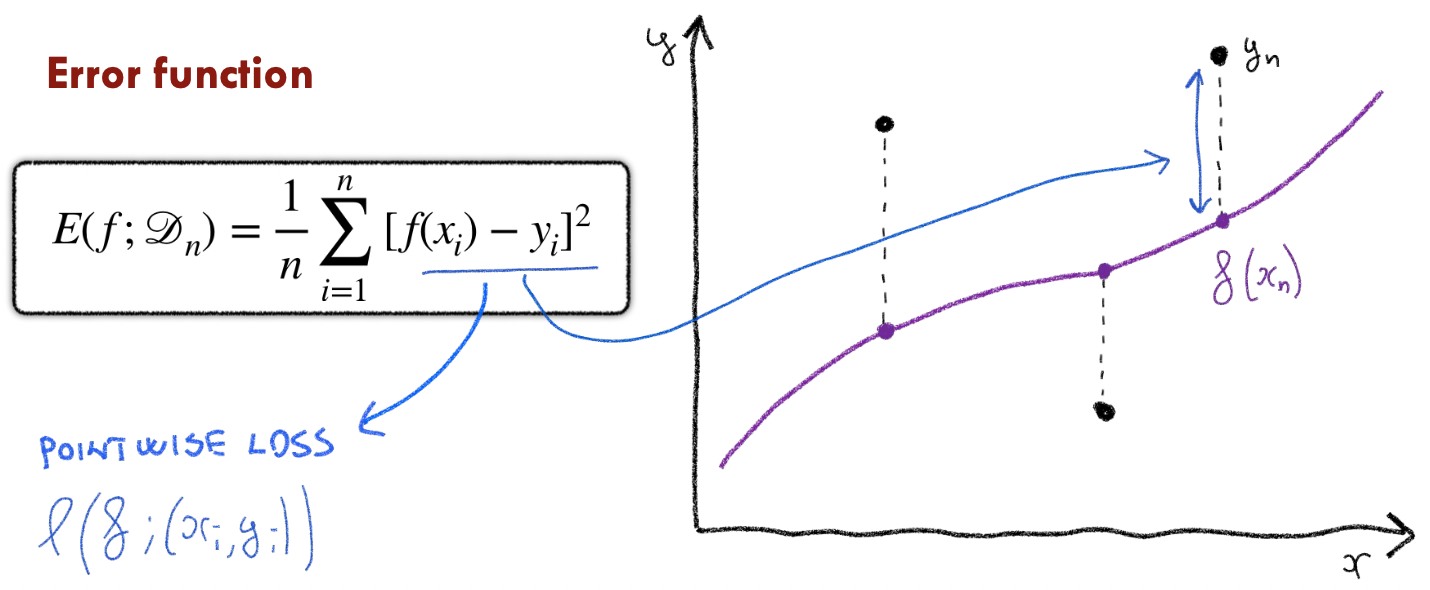
\includegraphics[width=0.7\textwidth]{../img/Mean_squared_error}
      \caption{Mean Squared Error}
\end{figure}

So, in the case of polynomial curve fitting, the best actual model would be
formalized as follows:

\begin{equation*}
      f_{\mathcal{H}_M}^*(\mathcal{D}_n) \in \arg \min_{f \in \mathcal{H}_M} E(f; \mathcal{D}_n)
\end{equation*}

which is actually equivalent to $f_{w^*}$ where $w^*$ is:

\begin{equation*}
      w^* \in \arg \min_{w \in \mathbb{R}^M} \frac{1}{n} \sum_{i = 1}^{n} [f_w(x_i) - y_i]^2
\end{equation*}

At this point, it is necessary to emphasize that the last equation mentioned
above \emph{can be actually computed} and in general only requires solving
a linear system of equations.

However, there is still one issue that has to be addressed. This issue consists
in the fact that, due to optimization difficulties encountered during the
execution of the learning algorithm, it might happen that the computed solution
is only a \emph{local minimum} $\hat{f}_{\mathcal{H}_M}^*(\mathcal{D}_n)$ and not a
\emph{global minimum} $f_{\mathcal{H}_M}^*(\mathcal{D}_n)$ that has been described
so far. This unfortunate issue can be observed in the following image:

\begin{figure}[h]
      \centering
      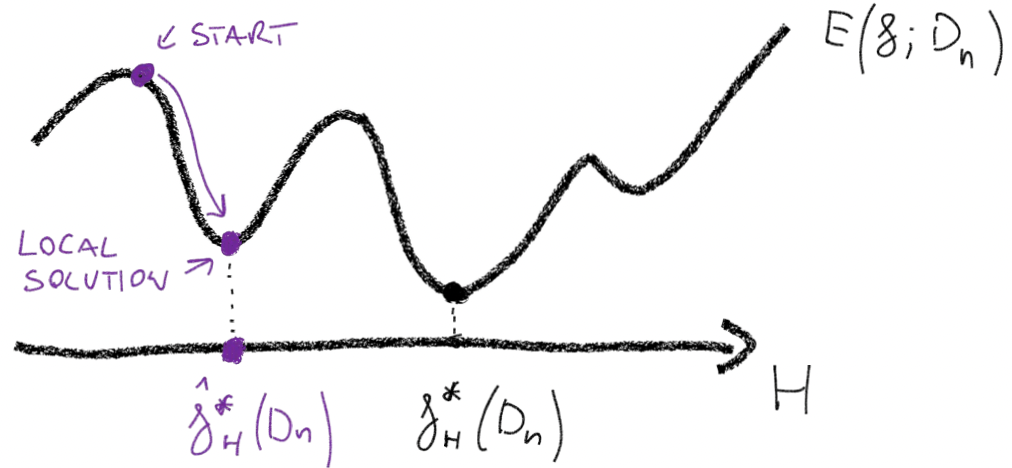
\includegraphics[width=0.65\textwidth]{../img/Best_local_actual_model}
      \caption{Local and Global Minima}
\end{figure}

So, at this point, it could be useful to summarize the differences between
all the different models that have been discussed so far by illustrating
them in the following image:

\newpage

\begin{figure}[h]
      \centering
      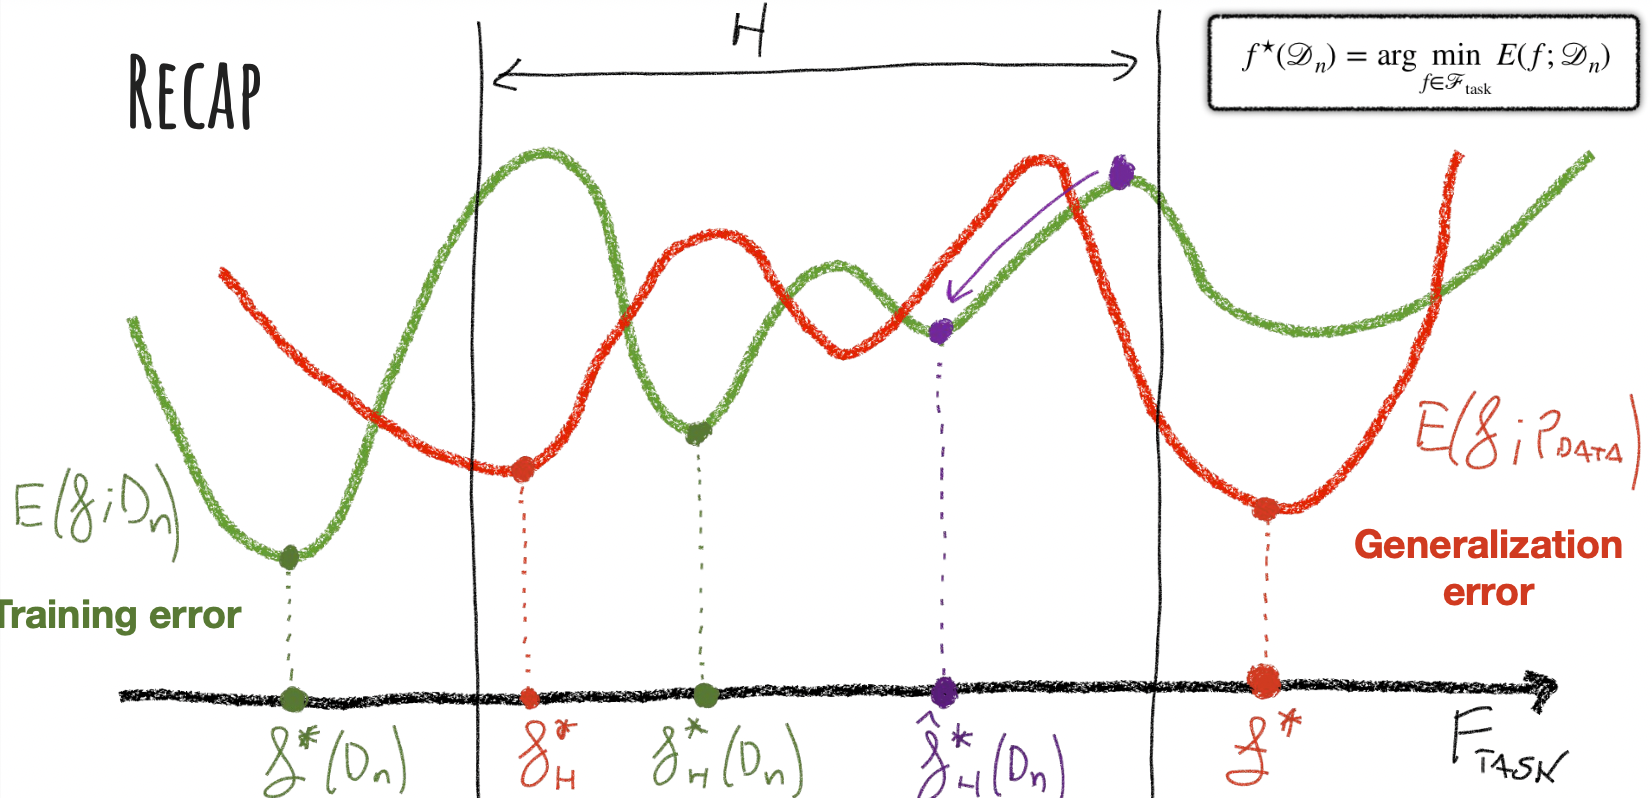
\includegraphics[width=0.7\textwidth]{../img/Recap_models}
      \caption{Summary of all types of models}
\end{figure}

At this point of this already long discussion about models, it is necessary to
talk about two other key concepts of machine learning that are \textbf{Underfitting}
and \textbf{Overfitting}:

\begin{itemize}
      \item \emph{\textbf{Underfitting}}: The situation of underfitting is observed
            when the value of the training error function is \emph{large}. This means
            that there is a big discrepancy between the accuracy of the model
            \emph{that has been computed} and the accuracy of the best model that
            \emph{can be computed} and that minimizes the training error. In other words,
            it is impossible to learn well enough from that particular training set.
            The concept of underfitting can be summarized by the following image:

            \begin{figure}[h]
                  \centering
                  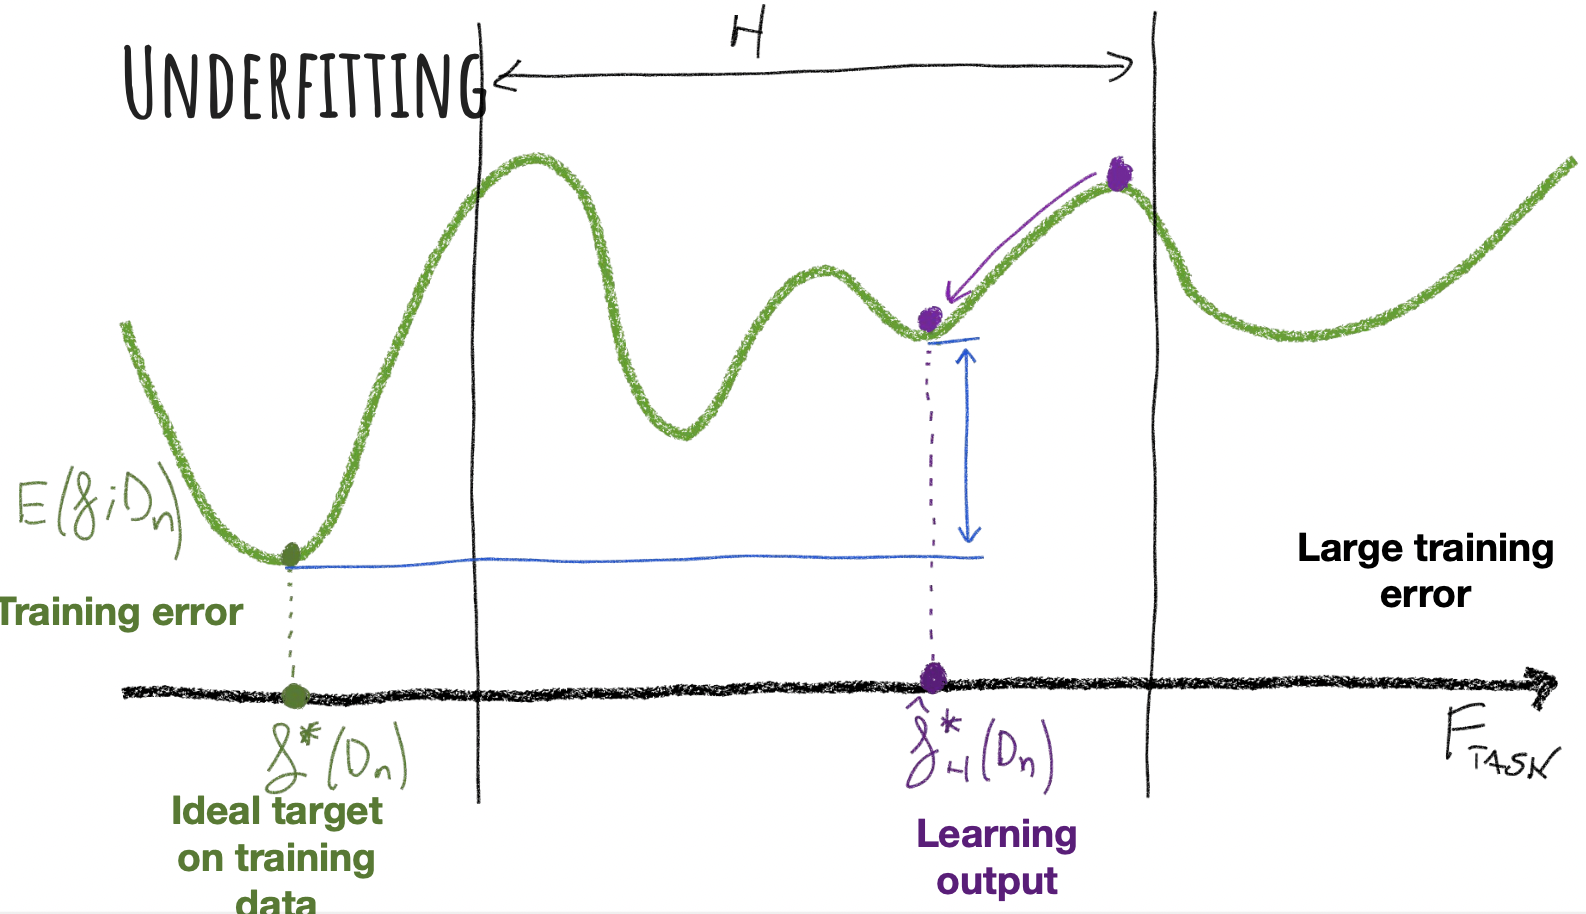
\includegraphics[width=0.65\textwidth]{../img/Underfitting}
                  \caption{Example of Underfitting}
            \end{figure}

      \item \emph{\textbf{Overfitting}}: The situation of overfitting is observed
            when the computed model has learned too well from a particular
            training set, so it performs exceptionally well on that dataset, but for
            this very reason there is a \emph{large generalization gap},
            which means that the model is not able to properly generalize to new
            unknown data, which are different from those seen in the training set.
            The concept of overfitting can be summarized by the following image:

            \newpage

            \begin{figure}[h]
                  \centering
                  \includegraphics[width=0.65\textwidth]{../img/Overfitting}
                  \caption{Example of Overfitting}
            \end{figure}

\end{itemize}

Now is the time to talk about other types of errors that are always present
and that depend on the choice of a particular training set, a particular
hypothesis space and the inherent variability of the predictions made on
new unknown data:

\begin{itemize}
      \item \emph{\textbf{Estimation Error}}: This is the error induced by learning
            on a \emph{particular data sample}. Therefore, it indicates the difference
            between the computed model and the best model in the hypothesis space that
            minimizes the generalization error. This difference can be observed
            in the following image:

            \begin{figure}[h]
                  \centering
                  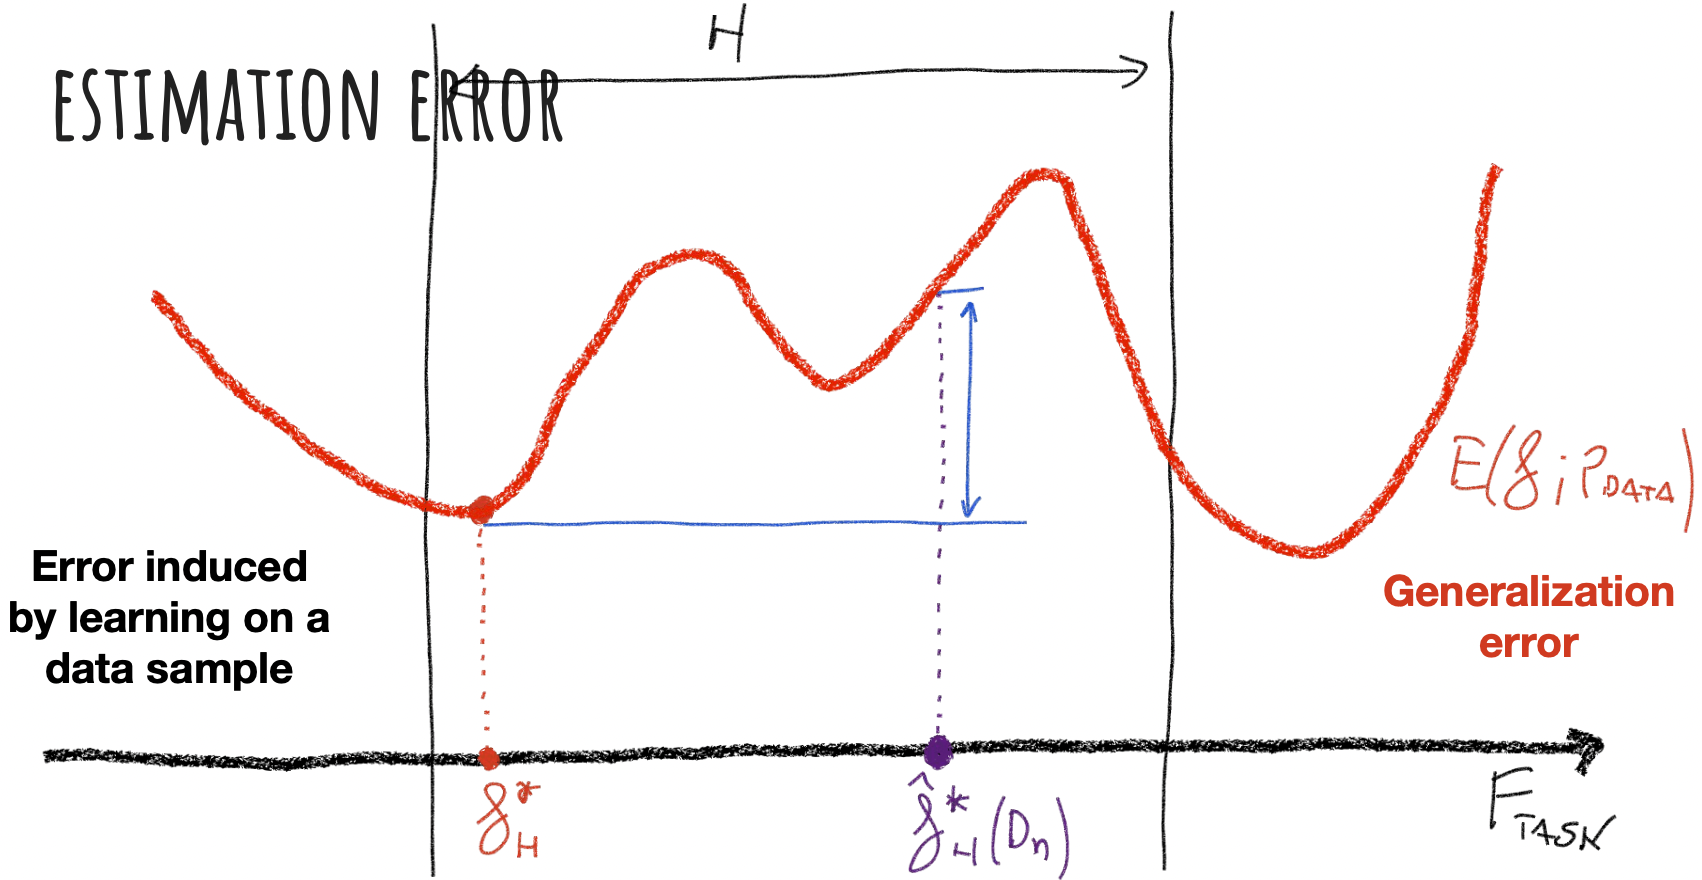
\includegraphics[width=0.65\textwidth]{../img/Estimation_error}
                  \caption{Example of Estimation Error}
            \end{figure}

      \item \emph{\textbf{Approximation Error}}: This is the error induced by the
            choice of \emph{a particular hypothesis space $\mathcal{H}$}. Therefore, it
            indicates the difference between the best model in the chosen hypothesis
            space that minimizes the generalization error and the best ideal model that
            minimizes the generalization error. This difference can be observed in the
            following image:

            \newpage

            \begin{figure}[h]
                  \centering
                  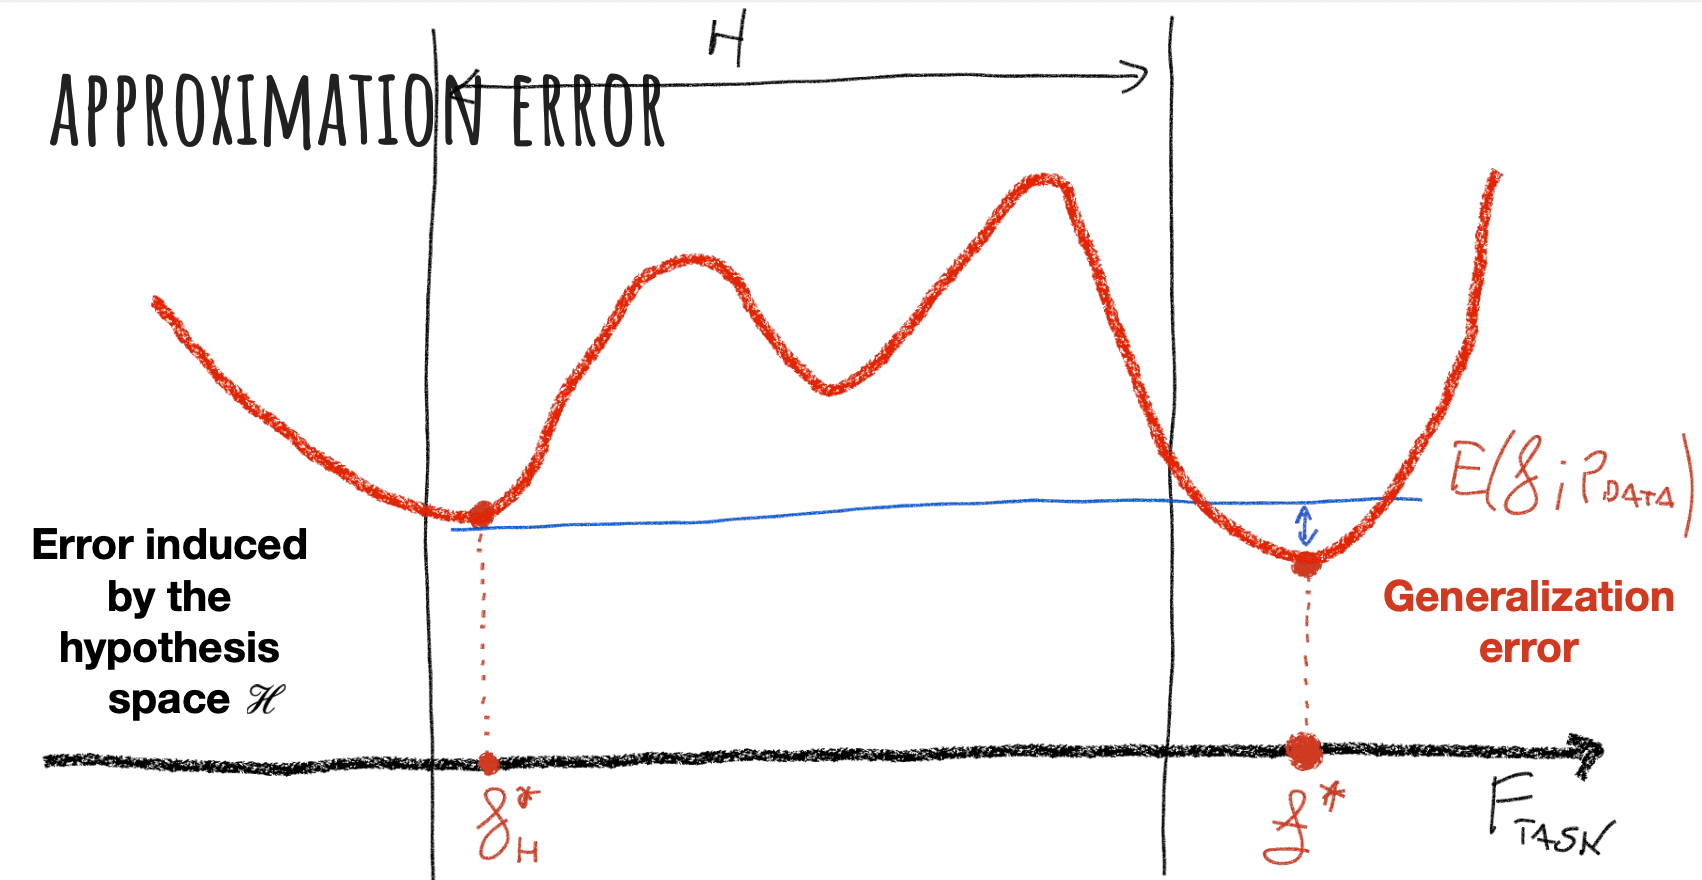
\includegraphics[width=0.65\textwidth]{../img/Approximation_error}
                  \caption{Example of Approximation Error}
            \end{figure}

      \item \emph{\textbf{Irreducible Error}}: This is the error due to the
            \emph{inherent data variability}. Therefore, it basically means that there
            will \emph{always} be some error between the predictions and the ground
            truths. This type of error can be observed in the following image:

            \begin{figure}[h]
                  \centering
                  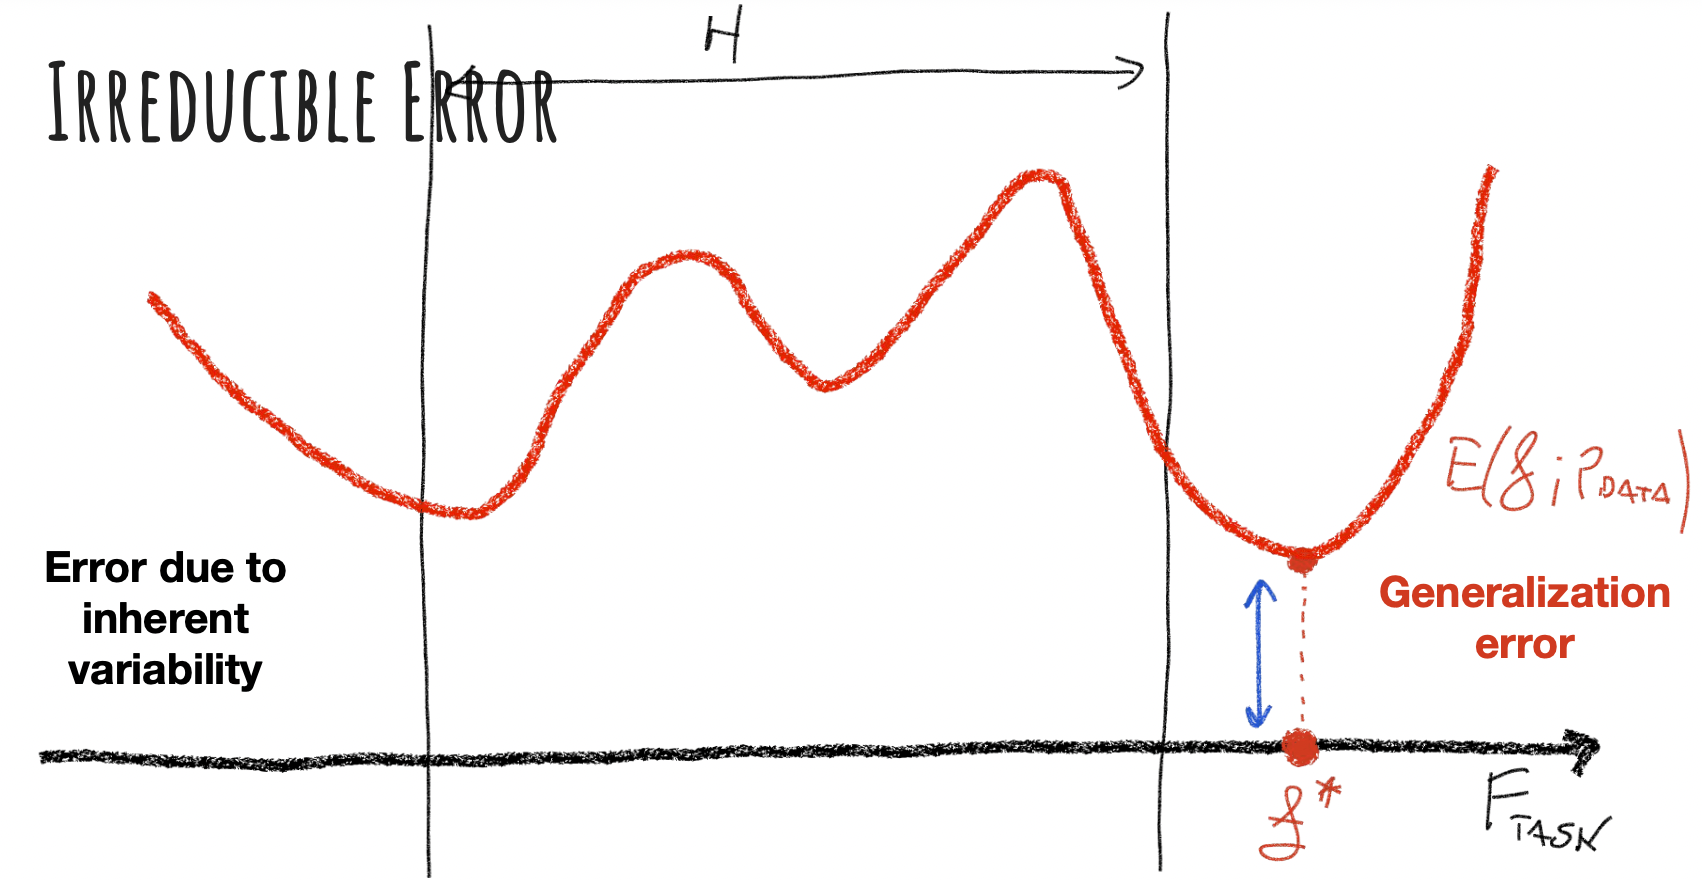
\includegraphics[width=0.65\textwidth]{../img/Irreducible_error}
                  \caption{Example of Irreducible Error}
            \end{figure}

\end{itemize}

At this point of reading, it is clear that the generalization error can not be computed
because the data generating distribution $p_{data}$ is unknown. Fortunately, it is
possible to approximately bypass this problem by using some data sampled from that
underlying distribution, so that, during the execution of the learning algorithm,
the training phase allows calculating the best model and the validation phase allows
calculating the best \emph{hyperparameters} for that model. Once this sequence of
operations has been performed, it is \textbf{assumed} that the training error
calculated on the final model should provide an acceptable estimation of the
generalization error. For this reason it is believed that this final model will perform
quite well on the test set. Therefore, it is possible, for example in the case of
polynomial curve fitting, to select the best model by considering the estimation of
the generalization error and by taking into account the concepts of underfitting
and overfitting, as can be observed in the following image:

\newpage

\begin{figure}[h]
      \centering
      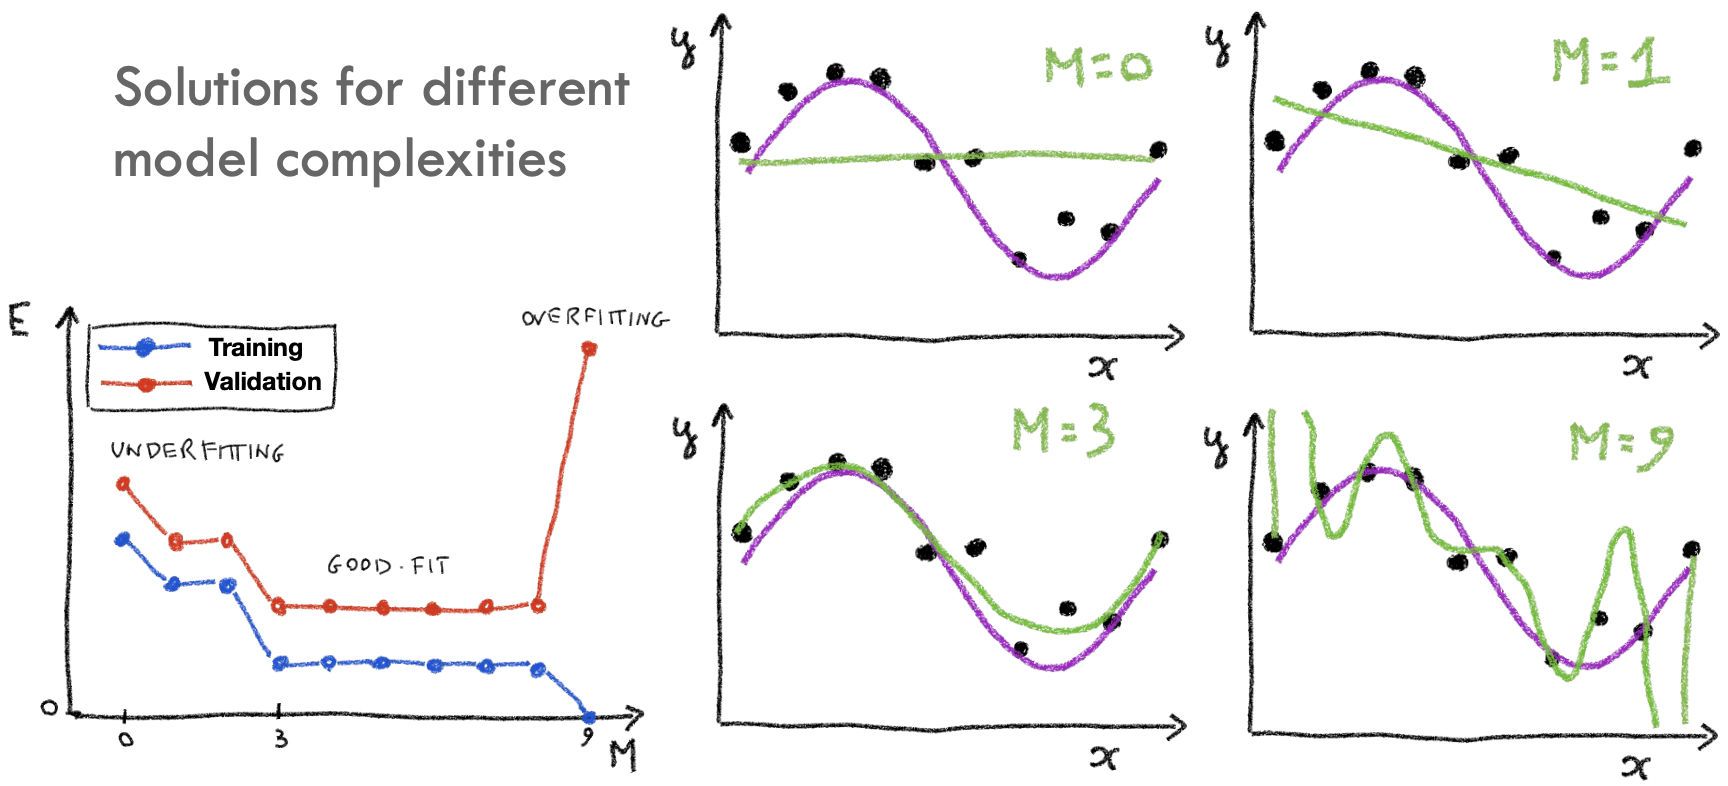
\includegraphics[width=0.9\textwidth]{../img/Model_selection}
      \caption{Example of Model Selection}
\end{figure}

However, it is becoming more and more interesting to understand how to improve
the generalization aspect of the model, and this can be done by considering
the following techniques, which will be discussed in more detail later in these notes:

\begin{itemize}
      \item \emph{\textbf{Minimal Training Error Avoidance}}: In general, it is
            recommended trying to avoid the minimal training error in order to avoid
            overfitting.
      \item \emph{\textbf{Model Capacity Reduction}}: In general, it is recommended
            reducing the capacity of the model in order to avoid overfitting, as can
            be observed in the image above in the case of a polynomial of degree 9.
      \item \emph{\textbf{Regularization}}: In this case, the objective function is
            integrated with a regularization term that allows penalizing solutions
            that are too complex and that tend to suffer from overfitting.
      \item \emph{\textbf{Noise Injection}}: By injecting some data noise into the
            learning algorithm, the model starts learning new features that
            will be useful for the future predictions.
      \item \emph{\textbf{Convergence Avoidance}}: In some cases, but especially
            in the case of a learning algorithm used to generate artificial neural
            networks, it is useful to stop the learning algorithm before it reaches the
            \emph{convergence}, which means that the final model will not learn too much
            from the training set and will probably be able to generalize more to the
            test set.
\end{itemize}

At this point, it is worth diving into the regularization approach mentioned above
to understand more in detail what it means to integrate the objective function
with a regularization term. It basically means to add to the objective function
$E(f; \mathcal{D}_n)$ a term $\lambda_n \Omega(f)$, where $\lambda_n$ is a
\textbf{hyperparameter} and is called \textbf{tradeoff parameter} because it
defines a tradeoff between the original objective function and the new term
in the sense that, by trading off both the objective function and the addictive term,
one chooses to be more addictive to the training data or to enforce generalization
to prevent overfitting. Therefore, the \emph{new} objective function becomes as follows:

\newpage

\begin{equation*}
      E_{reg}(f; \mathcal{D}_n) = E(f; \mathcal{D}_n) + \lambda_n \Omega(f)
\end{equation*}

\vspace{2mm}

and this concept can be observed even more clearly in the following image:

\begin{figure}[h]
      \centering
      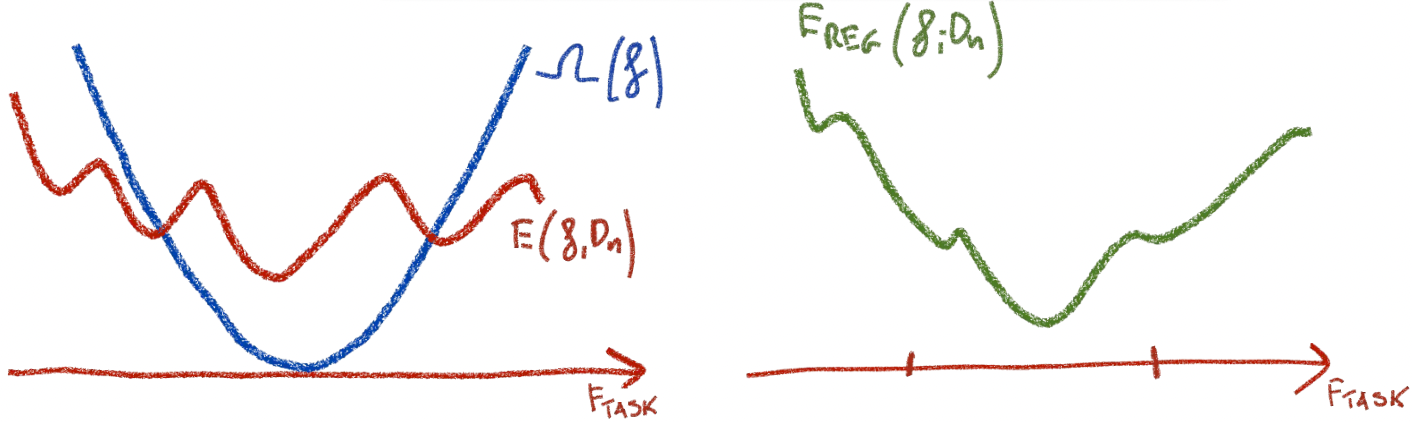
\includegraphics[width=0.9\textwidth]{../img/Regularization}
      \caption{Concept of Regularization}
\end{figure}

For example, in the case of polynomial curve fitting, one type of regularization
is called \textbf{L2 Norm Regularization}, where the sum of the squares of the
polynomial coefficients is minimized along with the original objective function,
so that polynomials with large coefficients are penalized. Therefore the training
error function becomes as follows:

\begin{equation*}
      E_{reg}(f_w; \mathcal{D}_n) = \frac{1}{n} \sum_{i = 1}^{n} [f_w(x_i) - y_i]^2 +
      \frac{\lambda}{n}{\left\lVert w\right\rVert}^2 \text{,} \ \text{where} \
      {\left\lVert w\right\rVert}^2 = \sum_{j = 1}^{M} w_j^2
\end{equation*}

\vspace{3mm}

and an example of this regularization can be observed in the following image:

\begin{figure}[h]
      \centering
      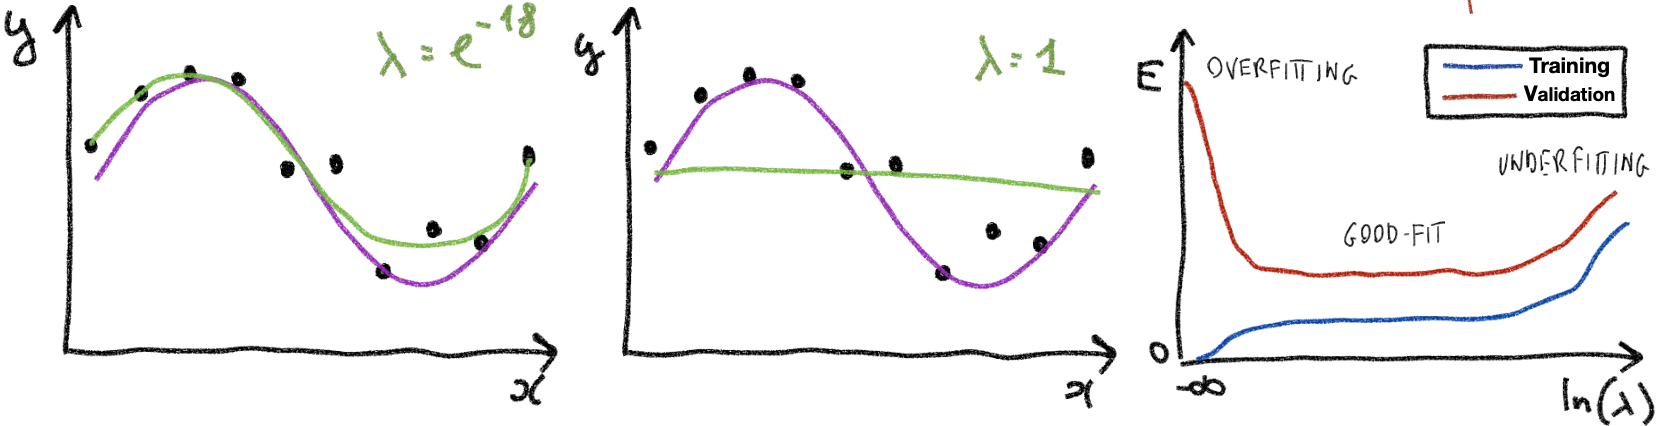
\includegraphics[width=0.9\textwidth]{../img/Regularization_PCF}
      \caption{Example of Regularization}
\end{figure}

where, the parameter $\lambda$ will be set by considering the performance of
the model on the validation set. In this image it is quite clear that the
parameter $\lambda$ somehow \emph{regulates} the tradeoff between overfitting
and underfitting, so that, for large values of $\lambda$, the model will tend
to underfit and, for very small values of $\lambda$, the model will tend to overfit.
Therefore, the right value for $\lambda$ will lie somewhere in between those
large and very small values.

However, there are also other techniques that can improve the generalization
ability of the final model and these techniques are the following:

\begin{itemize}
      \item \emph{\textbf{Increased Training Set Size}}: This basically means
            that the more training data are available the more likely it is that
            the final model will be able to generalize to new unknown data.
            Unfortunately, this is not always possible.
      \item \emph{\textbf{Data Augmentation}}: This approach suggests
            \emph{augmenting} the training set by applying some random
            \emph{transformations}(in the case of images these can be flips
            and rotations) to the data already available in the training set
            in order to produce new data that will hopefully make the final
            model more capable of generalizing.
      \item \emph{\textbf{Ensemble Learning}}: This approach suggests
            combining the predictions of multiple, uncorrelated models
            during the test phase in order to have a combined prediction
            that will probably provided a better result.
\end{itemize}

As the last deepening of this long and complicated subsection, it is worth
diving into the increased training set size approach where the size of the
training set is increased to improve the generalization capability. This
approach is quite interesting since, even if the model flexibility is
high(as in the case of polynomial curve fitting where the polynomial degree
is high), the training set is also very large, so the overall model is quite
accurate. The reason why this happens is that, as the size of the available
data increases, the training error tends to become more and more similar to
the generalization error, such that the following relation is obtained:

\begin{equation*}
      E(f; \mathcal{D}_n) \rightarrow
      E(f; p_{data}) \ \text{as} \ n \rightarrow \infty
\end{equation*}

\vspace{3mm}

This result can be observed even more clearly in the following image:

\begin{figure}[h]
      \centering
      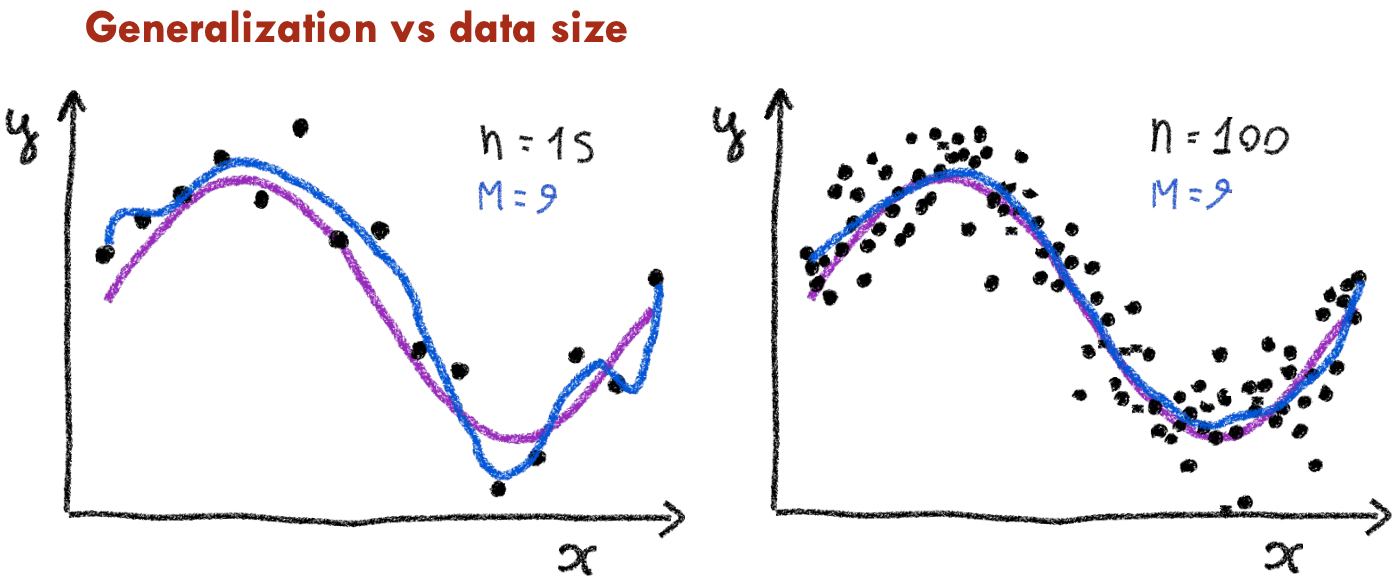
\includegraphics[width=0.8\textwidth]{../img/Generalization_vs_data_size}
      \caption{Generalization vs Data Size}
\end{figure}

At this point, there should be a discussion about learning algorithms,
however, since the number of these learning algorithms is considerably
large, it is better to postpone this discussion to the next section.
